\documentclass[
    12pt,
    oneside,
    a4paper,
    english,
    brazil,
    sumario=tradicional,
    msc
]{dcomp-abntex2}

\microtypesetup{expansion=false}

\usepackage[T1]{fontenc}
\usepackage{lmodern}
\usepackage{graphicx}
\usepackage{float}
\usepackage{amsmath}
\usepackage{booktabs}
\usepackage{multirow}
\usepackage{array}
\usepackage{url}
\usepackage{lipsum}

% ---------------------------------------------------
% Informações da proposta
% ---------------------------------------------------
\titulo{Democratizando o Acesso à Informação Legislativa: Inteligência Artificial Generativa para Análise de Dados Parlamentares}
\autor{Ana Beatriz Carvalho Oliveira}
\local{São Cristóvão -- Sergipe}
\data{2026} % Atualizei para 2026, já que a defesa/qualificação virou o ano
\orientador{Prof. Dr. Gilton José Ferreira da Silva}
\curso{Ciência da Computação}
\instituicao{%
  Universidade Federal de Sergipe\\
  Centro de Ciências Exatas e Tecnologia\\
  Programa de Pós-Graduação em Ciência da Computação
}
\tipotrabalho{Proposta de Dissertação}

% ---------------------------------------------------
\begin{document}
\imprimircapa
\imprimirfolhaderosto*

% ---------------------------------------------------
% Elementos pré-textuais
% ---------------------------------------------------

% --- RESUMO EM PORTUGUÊS ---
\begin{resumo}
A crescente produção de dados brutos pelo Senado Federal impõe desafios à sua organização, consulta e interpretação, limitando a efetividade da transparência pública. Este trabalho insere-se nesse contexto, adotando a metodologia \textit{Design Science Research} (DSR) para investigar a aplicação de Inteligência Artificial Generativa na análise de dados parlamentares abertos. O objetivo é projetar, desenvolver e avaliar tecnicamente um artefato computacional capaz de estruturar dados legislativos, classificar discursos e apoiar consultas em linguagem natural. A solução proposta, denominada AgentAI, consiste em uma aplicação \textit{web} interativa que automatiza a extração de dados da API do Senado e utiliza o modelo Mistral 7B Instruct executado localmente para classificação temática e geração de respostas ancoradas nos dados recuperados. A avaliação será conduzida sem coleta de dados com participantes humanos, por meio de cenários representativos de consulta, comparação com gabaritos de referência, verificação de rastreabilidade e análise factual das respostas. O artefato encontra-se funcional e já passou por verificação funcional preliminar; esta proposta detalha o protocolo de avaliação científica --- classificação temática, coerência factual e rastreabilidade ---, cuja execução constitui a etapa em andamento. A pesquisa investiga em que medida a combinação entre dados abertos, IA Generativa local e interfaces visual/conversacional pode reduzir barreiras cognitivas e técnicas de acesso à informação legislativa.

\textbf{Palavras-chave}: Inteligência Artificial Generativa. Dados Abertos. Design Science Research. Transparência Pública. Processamento de Linguagem Natural.
\end{resumo}

% --- RESUMO EM INGLÊS ---
\begin{resumo}[Abstract]
The growing production of raw data by the Federal Senate poses challenges to organization, querying, and interpretation, limiting the effectiveness of public transparency. Within this context, this work adopts the Design Science Research (DSR) methodology to investigate the application of Generative Artificial Intelligence in the analysis of open parliamentary data. The objective is to design, develop, and technically evaluate a computational artifact capable of structuring legislative data, classifying speeches, and supporting natural-language queries. The proposed solution, named AgentAI, consists of an interactive web application that automates data extraction from the Senate API and uses the locally executed Mistral 7B Instruct model for thematic classification and data-grounded response generation. The evaluation will be conducted without collecting data from human participants, using representative query scenarios, comparison with reference answers, traceability checks, and factual analysis of generated responses. The artifact is functional and has undergone preliminary functional verification; this proposal details the scientific evaluation protocol --- thematic classification, factual coherence, and traceability ---, whose execution constitutes the ongoing stage. The research investigates to what extent combining open data, local Generative AI, and visual/conversational interfaces can reduce cognitive and technical barriers to accessing legislative information.

\textbf{Keywords}: Generative Artificial Intelligence. Open Data. Design Science Research. Public Transparency. Natural Language Processing.
\end{resumo}

% --- LISTAS ---

\cleardoublepage
\listoffigures*

\cleardoublepage
\listofquadros*

\cleardoublepage
\tableofcontents*

% ---------------------------------------------------
% Elementos textuais
% ---------------------------------------------------
% DICA: Lembre-se de atualizar o conteúdo dentro dos arquivos .tex abaixo
% para refletir a mudança para Design Science Research e a nova Questão de Pesquisa.

\chapter{Introdução}
A crescente abertura de dados governamentais no Brasil criou um paradoxo pouco discutido: os dados estão tecnicamente disponíveis, mas permanecem inacessíveis para a maior parte da população. Esta dissertação parte desse problema concreto para investigar se — e em que medida — a Inteligência Artificial Generativa pode reduzir essa distância entre disponibilidade técnica e acesso efetivo à informação parlamentar.

\section{Contexto}
A busca por um governo transparente é um pilar fundamental da democracia, onde a visibilidade do poder legitima as instituições \cite{Bobbio1986}. No século XXI, essa premissa é potencializada pelo movimento de dados abertos (Open Data), que defende que os dados governamentais devam ser livremente utilizados, reutilizados e redistribuídos \cite{OKBrasil2024}. Contudo, a simples disponibilização das informações sobre as atividades parlamentares não assegura, por si só, a efetividade da transparência. A proliferação de dados brutos, como os debates e discursos políticos, requer métodos de organização, recuperação e análise para que a informação pública possa ser consultada de modo inteligível — pois, como argumentam \citeonline{OliveiraCkagnazaroff2022}, a transparência efetiva exige que os dados sejam não apenas públicos, mas também claros, contextualizados e utilizáveis. Quando essa mediação não se realiza, o fosso entre o que está formalmente disponível e o que é efetivamente acessível contribui para aprofundar o distanciamento entre representados e representantes — condição que \citeonline{LevitskyZiblatt2018} identificam como uma das precursoras do enfraquecimento das instituições democráticas. Nesse cenário, a Inteligência Artificial (IA), com destaque para a IA Generativa, apresenta potencial para processar, classificar e sintetizar grandes volumes de dados textuais, apoiando novas formas de consulta à informação pública.

\section{Motivação}
A motivação central deste trabalho está na distância entre o que os dados parlamentares abertos prometem e o que efetivamente entregam. A API do Senado Federal disponibiliza volumes crescentes de informações sobre sessões, discursos e votações, mas consultá-la exige familiaridade com estruturas técnicas (endpoints, formatos XML/JSON) que escapam ao repertório da maioria dos cidadãos. Não se trata de um problema de vontade política na abertura dos dados — trata-se de um problema de mediação entre dado bruto e informação compreensível. A aplicação da IA Generativa nesse contexto não é uma solução trivial: ela carrega consigo riscos conhecidos de imprecisão factual e viés algorítmico que precisam ser investigados antes de qualquer uso em contextos cívicos. É exatamente essa tensão — potencial de democratização versus riscos de desinformação — que motiva a pesquisa aqui proposta.

O artefato desenvolvido nesta dissertação, denominado \textit{AgentAI}, é uma aplicação web que integra coleta automatizada de dados parlamentares via API do Senado Federal, classificação temática de discursos com IA Generativa executada localmente, visualizações interativas e um agente conversacional para consultas em linguagem natural. A escolha por execução local — em vez de APIs proprietárias — responde a critérios científicos concretos: replicabilidade do experimento, soberania dos dados e independência de custos operacionais.

\section{Problemática, Questão de Pesquisa e Hipótese}

\subsection{Problemática}
A principal problemática abordada decorre do fato de que o volume e a complexidade dos dados parlamentares abertos, embora publicamente disponíveis, representam uma barreira significativa para consulta e análise. Como discutido por \citeonline{OliveiraCkagnazaroff2022}, para que a transparência seja efetiva, os dados devem ser não apenas públicos, mas também claros, contextualizados e utilizáveis. Atualmente, a análise proficiente desses dados exige conhecimentos técnicos, familiaridade com as estruturas das APIs e o dispêndio de tempo considerável.

Complementarmente, \citeonline{Lee2017}, através do VLAT (\textit{Visualization Literacy Assessment Test}), demonstraram que a interpretação das visualizações gráficas pode variar conforme a literacia visual dos usuários. \citeonline{Hornung2015} apontam que as pessoas sem formação em estatística ou ciência de dados podem enfrentar barreiras cognitivas ao analisar os dados complexos. Portanto, a mera disponibilização dos dados legislativos não garante, por si só, que essas informações sejam facilmente consultáveis ou compreensíveis.

Nesse contexto, a Inteligência Artificial Generativa, exemplificada pelos modelos como o Mistral 7B Instruct \cite{MistralAI2024}, apresenta-se como uma abordagem promissora para apoiar a organização e a consulta dos dados legislativos textuais. Diferentemente das técnicas tradicionais de Processamento de Linguagem Natural (PLN) que dependem de palavras-chave rígidas, os modelos de linguagem podem apoiar tarefas de classificação temática, sumarização e geração de respostas em linguagem natural. A execução local do modelo também contribui para a privacidade, replicabilidade e independência das APIs proprietárias.

\subsection{Questão de Pesquisa}
Diante desse cenário, este trabalho norteia-se pela seguinte questão de pesquisa central:

\begin{citacao}
\textbf{QP:} Em que medida um artefato computacional baseado em \textit{dashboard} visual e agente conversacional com IA Generativa local pode estruturar, classificar e tornar consultáveis os dados parlamentares abertos do Senado Federal?
\end{citacao}

\subsection{Hipótese de Pesquisa}
Para responder a esta questão, foi formulada a seguinte hipótese de trabalho:

\begin{citacao}
\textbf{Hipótese:} A combinação do processamento dos dados abertos, classificação temática com o Mistral 7B Instruct e interface visual/conversacional é capaz de estruturar e tornar consultáveis dados parlamentares abertos, de modo que: (a) a classificação temática automática dos discursos apresente acurácia superior à de um classificador por palavras-chave utilizado como linha de base; (b) as respostas do agente conversacional sejam factualmente coerentes com os dados recuperados em pelo menos 70\% dos cenários de consulta avaliados; e (c) as respostas apresentem rastreabilidade explícita — isto é, possam ser associadas aos registros de origem — em pelo menos 80\% dos casos. Caso esses limiares não sejam alcançados, a hipótese será refutada e as causas do insucesso constituirão o principal resultado científico da dissertação.
\end{citacao}

\section{Objetivos}

\subsection{Objetivo Geral}
Investigar como a aplicação da Inteligência Artificial Generativa local nos dados legislativos abertos pode apoiar a estruturação, classificação e consulta das informações parlamentares, mediante o design, implementação e avaliação técnica de um artefato computacional interativo que integra interface visual e conversacional.

\subsection{Objetivos Específicos}
Para que o objetivo geral seja alcançado, foram definidos os seguintes objetivos específicos, alinhados às etapas da metodologia \textit{Design Science Research}:

\begin{itemize}
\item Realizar um mapeamento sistemático da literatura para identificar os fundamentos teóricos sobre os dados abertos, IA Generativa em contextos cívicos, interação humano-dados e consulta aos dados legislativos.
\item Descrever e justificar os fundamentos teóricos para as escolhas de design do artefato, especificamente a combinação do \textit{dashboard} visual e agente conversacional baseado na IA Generativa local.
\item Implementar um protótipo funcional (\textit{artefato computacional}) capaz de processar os dados legislativos abertos da API do Senado Federal, classificar tematicamente os discursos e responder às perguntas em linguagem natural utilizando o modelo Mistral 7B Instruct.
\item Avaliar a eficácia técnica do artefato, verificando a qualidade da coleta e estruturação dos dados, a acurácia da classificação temática e a qualidade factual das respostas geradas em comparação com os dados oficiais.
\item Avaliar a rastreabilidade das respostas geradas pelo agente conversacional, verificando se as informações apresentadas podem ser associadas aos dados recuperados, como discurso, votação, data, parlamentar ou matéria legislativa.
\item Documentar o conhecimento científico gerado sobre o design e a avaliação dos artefatos computacionais para consulta aos dados parlamentares abertos com IA Generativa local.
\end{itemize}

\section{Estrutura do Documento}

O documento está organizado em seis capítulos. A Fundamentação Teórica (Cap. 2) apresenta os conceitos de dados abertos, PLN, IA Generativa, RAG, DSR e interação humano-dados. A Metodologia (Cap. 3) detalha as seis fases DSR e o protocolo de avaliação do artefato. O Estado da Arte (Cap. 4) mapeia sistematicamente a literatura existente e posiciona esta pesquisa em relação ao campo. O Desenvolvimento (Cap. 5) descreve a arquitetura do AgentAI e os resultados preliminares. As Considerações Parciais (Cap. 6) analisam o progresso alcançado, os desafios identificados e as perspectivas de conclusão.

A adjacência intencional entre os capítulos de Metodologia e Estado da Arte permite que o leitor conheça primeiro as decisões metodológicas adotadas — inclusive o protocolo de avaliação — para então confrontá-las com as práticas documentadas pela literatura, tornando explícita a contribuição original desta dissertação.


\chapter{Fundamentação Teórica}
\section{Dados Abertos}

Este trabalho se fundamenta na disponibilização de dados governamentais em formato aberto, livre de restrições de direitos autorais ou outros mecanismos de controle. Conforme definido pelo movimento OK Brasil \cite{OKBrasil2024} e pelo Arquivo Nacional do Reino Unido \cite{ArquivoNacional2023}, os "dados abertos" são aqueles disponibilizados livremente para acesso, uso, reutilização e redistribuição por qualquer indivíduo. Para que sejam considerados como tal, é crucial que os dados estejam em formatos abertos e não proprietários, permitindo a sua fácil integração com outros sistemas e ferramentas.

No contexto da pesquisa científica, os dados abertos são essenciais para a aceleração de descobertas e a promoção da colaboração \cite{SayaoSales2014}. Ao tornar dados disponíveis em formato aberto, pesquisadores e cientistas sociais ganham condições concretas para replicar estudos, contestar resultados e explorar perspectivas de análise que dependem do acesso livre a fontes primárias. Sayão e Sales \cite{SayaoSales2014} argumentam que essa abertura não é apenas uma mudança técnica, mas uma transformação nas práticas de comunicação científica, exigindo novas formas de gerenciamento, preservação e compartilhamento de dados ao longo do tempo.

Na gestão pública, os dados abertos são fundamentais para a transparência e a accountability. Ao disponibilizar dados sobre gastos públicos e contratos governamentais, os governos aumentam sua transparência e permitem um controle social mais rigoroso \cite{ZuiderwijkJanssen2014}. No Brasil, a API do Senado Federal configura-se como uma ferramenta essencial para a democracia participativa, oferecendo dados brutos sobre o funcionamento da Instituição. Contudo, a efetividade dessa abertura depende da qualidade com que os dados são entregues aos cidadãos. Conforme argumentado por Vetro et al. \cite{Vetro2016}, a qualidade dos dados deve ser observada em todas as etapas de sua disponibilização, desde a coleta até a apresentação. A Figura \ref{fig:processo_publicacao} ilustra o processo de publicação de dados abertos e os pontos críticos onde a intervenção técnica é necessária para assegurar que o dado bruto se torne informação útil.

\begin{figure}[H]
\centering
\caption{Processo de publicação e estruturação de dados abertos}
\label{fig:processo_publicacao}
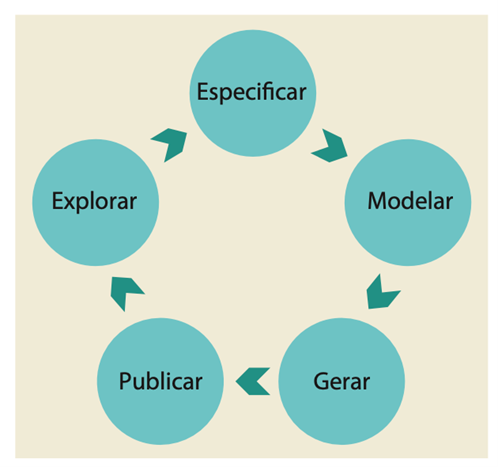
\includegraphics[width=0.6\textwidth]{imagens/publicacao.png}
\fonte{Adaptado de Villazón-Terrazas et al. (2011).}
\end{figure}

\subsection{As 5 Estrelas dos Dados Abertos}

Para maximizar o potencial de reutilização e interoperabilidade dos dados abertos, Tim Berners-Lee propôs um sistema de classificação de 5 estrelas (Figura \ref{fig:5_estrelas}), que gradua o nível de abertura e estruturação dos dados \cite{IsotaniBittencourt2015}. A seguir, são descritas cada uma das etapas:

\begin{itemize}
\item \textbf{1 estrela:} Disponível na web (qualquer formato) com licença aberta. Este é o nível mais básico de abertura de dados.
\item \textbf{2 estrelas:} Disponível como dados estruturados (por exemplo, em formatos CSV ou Excel). Nesse estágio, os dados são organizados em tabelas ou outras estruturas que facilitam a sua manipulação e análise.
\item \textbf{3 estrelas:} Como 2 estrelas, mas em formato não proprietário. Aqui, os dados estão disponíveis em formatos abertos padronizados (como CSV), o que facilita sua integração com diversas ferramentas de visualização e análise.
\item \textbf{4 estrelas:} Como 3 estrelas, mais uso de URIs e padrões W3C (RDF, SPARQL). Neste estágio, os dados são identificáveis na web através de URIs, o que permite a sua ligação com outras fontes de informação. Os dados também podem ser descritos em formato RDF, permitindo a sua integração com recursos semânticos padronizados.
\item \textbf{5 estrelas:} Como 4 estrelas, mais ligação (link) com outros dados para fornecer contexto (\textit{Linked Data}). Neste ponto, os dados não apenas são abertos e interoperáveis, mas também estão conectados a outras fontes de informação relevantes. Isso permite a construção de aplicações que fornecem uma visão holística dos dados.
\end{itemize}

\begin{figure}[H]
\centering
\caption{Diagrama das 5 estrelas de Dados Abertos}
\label{fig:5_estrelas}
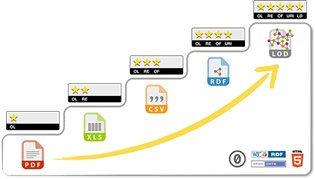
\includegraphics[width=0.8\textwidth]{imagens/estrelas.png}
\fonte{5stardata.info.}
\end{figure}

\section{Processamento de Linguagem Natural (PLN) e Modelos de Linguagem}

O Processamento de Linguagem Natural (PLN) é uma subárea da Inteligência Artificial que se dedica a capacitar os computadores para processar e compreender a linguagem humana \cite{JurafskyMartin2023}. A abordagem clássica do PLN exigia um \textit{pipeline} complexo de pré-processamento manual e intensivo (Figura \ref{fig:pln_classico}), onde o texto era convertido em representações vetoriais numéricas.

\begin{figure}[H]
\centering
\caption{Abordagem Clássica de PLN}
\label{fig:pln_classico}
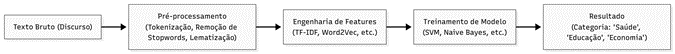
\includegraphics[width=0.8\textwidth]{imagens/abordagem_pln.png}
\fonte{Produção da autora.}
\end{figure}

Com o advento dos Modelos de Linguagem de Larga Escala (LLMs), essa abordagem mudou drasticamente. Como ilustrado na Figura \ref{fig:pln_generativo}, os LLMs são capazes de realizar tarefas complexas, como tradução, resumo e geração de texto, de forma \textit{end-to-end}, sendo instruídos por comandos em linguagem natural (\textit{prompts}).

\begin{figure}[H]
\centering
\caption{Abordagem Generativa com LLMs}
\label{fig:pln_generativo}
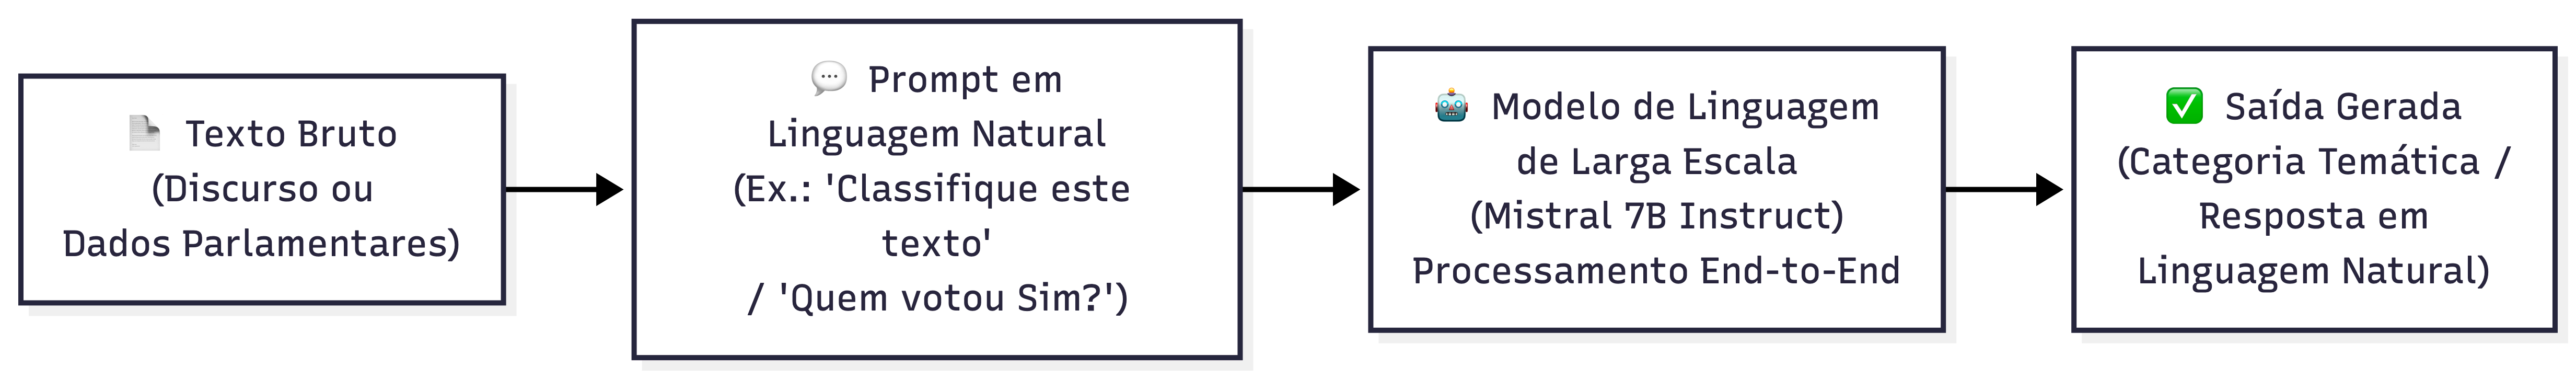
\includegraphics[width=0.8\textwidth]{imagens/abordagem_generativa.png}
\fonte{Produção da autora.}
\end{figure}

Este trabalho adota a abordagem generativa, utilizando o modelo Mistral 7B Instruct \cite{MistralAI2024}, que roda em ambiente local para executar tarefas de classificação temática e resposta a perguntas (\textit{Question Answering}), dispensando a necessidade de treinamento de modelos específicos para cada tarefa e evitando dependência de APIs externas.

\section{Inteligência Artificial Generativa}

Os Modelos de Linguagem de Larga Escala (LLMs) são modelos fundamentados em arquiteturas de redes neurais profundas (\textit{deep learning}), treinados com volumes massivos de dados para compreender e gerar linguagem com alta fluência \cite{RedHat2023}. O fluxo típico de desenvolvimento desses modelos envolve coleta, treinamento e refinamento por \textit{feedback} humano (RLHF), conforme a Figura \ref{fig:fluxo_llm}.

\begin{figure}[H]
\centering
\caption{Fluxo de Treinamento e Refinamento de um LLM}
\label{fig:fluxo_llm}
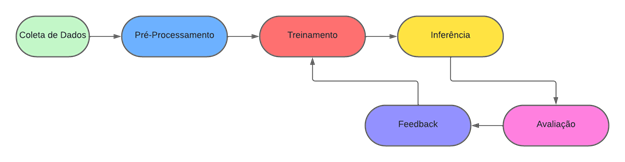
\includegraphics[width=0.8\textwidth]{imagens/llm.png}
\fonte{Produção da autora.}
\end{figure}

No contexto desta pesquisa, a IA Generativa é empregada para classificar discursos parlamentares por tema e gerar respostas em linguagem natural a partir de dados legislativos estruturados \cite{Tamper2022}. Esse uso, porém, não é isento de riscos: alucinações — respostas factualmente incorretas geradas com aparente confiança pelo modelo — e vieses presentes nos dados de treinamento representam ameaças concretas à confiabilidade do sistema \cite{MarquesLaipelt2023}. Em contextos cívicos, onde informação imprecisa pode influenciar a percepção pública sobre representantes políticos, esses riscos não podem ser tratados apenas como limitações técnicas; eles exigem mecanismos explícitos de verificação e rastreabilidade, que constituem, precisamente, um dos focos desta dissertação.

\subsection{Recuperação Aumentada por Geração}

Além da geração textual, este trabalho adota uma estratégia de Recuperação Aumentada por Geração (\textit{Retrieval-Augmented Generation} -- RAG). Em linhas gerais, RAG combina uma etapa de recuperação de informações relevantes em uma base de dados ou coleção documental com uma etapa de geração de resposta por modelo de linguagem \cite{Lewis2020}. Essa abordagem é adequada para domínios em que a resposta deve permanecer ancorada em fontes verificáveis, pois o modelo não responde apenas com base em seus parâmetros internos: ele recebe, no \textit{prompt}, um contexto recuperado previamente.

No AgentAI, a etapa de recuperação não emprega indexação vetorial densa com modelos de \textit{embedding} e operações de similaridade semântica, mas sim \textbf{busca estruturada} sobre a base local --- filtrando registros por parlamentar, período, tema ou palavras presentes no texto --- e fornece esse contexto diretamente ao Mistral 7B Instruct para a geração da resposta. Por rigor terminológico, esta dissertação refere-se a tal estratégia como \textit{recuperação estruturada com geração aumentada} (uma abordagem inspirada em RAG), reservando o termo RAG, em sentido estrito \cite{Lewis2020}, para arquiteturas que realizam recuperação por similaridade semântica densa. Essa escolha implica um \textit{trade-off} explícito: perde-se a capacidade de recuperar documentos por paráfrase ou sinônimo (limitação que será documentada na avaliação), mas ganha-se rastreabilidade direta --- cada resposta pode ser associada aos registros exatos que a fundamentaram. Para o objetivo desta dissertação, que é justamente investigar a qualidade factual e a rastreabilidade das respostas em contexto legislativo, essa abordagem é metodologicamente coerente.

\subsection{Mistral 7B Instruct vs. Alternativas}
\label{subsec:escolha_modelo}

A escolha do modelo Mistral 7B Instruct justifica-se por múltiplos aspectos técnicos e científicos. Diferentemente de APIs proprietárias como Google Gemini, Mistral 7B oferece:

\begin{itemize}
\item \textbf{Privacidade e Soberania de Dados:} O modelo roda localmente, garantindo que os dados legislativos brasileiros não sejam transmitidos para servidores externos, o que se alinha com princípios de soberania digital.
\item \textbf{Replicabilidade:} Por ser \textit{open-source}, permite que outros pesquisadores reproduzam exatamente o experimento e validem os resultados de forma independente, atendendo aos critérios de rigor científico.
\item \textbf{Custo Operacional:} Elimina dependência de APIs pagas, reduzindo barreiras financeiras para a replicação da pesquisa.
\item \textbf{Performance Adequada:} Apesar de menor em parâmetros que os grandes modelos proprietários, o Mistral 7B Instruct apresenta desempenho competitivo em tarefas de compreensão e geração de linguagem em benchmarks gerais \cite{Jiang2023}; sua adequação específica ao domínio legislativo em português constitui, precisamente, uma das questões investigadas nesta dissertação.
\end{itemize}

Este trade-off entre capacidade absoluta (modelos proprietários maiores) e replicabilidade (modelo local open-source) representa uma escolha metodológica consciente que prioriza a sustentabilidade e transparência da pesquisa.

Reconhece-se que o Mistral 7B Instruct, lançado em 2023, não é o modelo aberto mais recente disponível ao tempo de conclusão desta dissertação. A escolha, contudo, prioriza deliberadamente a \textbf{replicabilidade} sobre a recência: um modelo congelado, amplamente documentado e de pesos abertos permite que o experimento seja reproduzido de forma idêntica por terceiros --- garantia que não se obtém com modelos sujeitos a atualizações frequentes ou a descontinuação. Trata-se, portanto, de uma limitação assumida, e não de uma afirmação de superioridade do modelo. Essa opção é viabilizada pela arquitetura modular do artefato quanto ao componente de linguagem: o LLM é acessado por uma interface de inferência padronizada, de modo que a substituição por um modelo mais recente constitui trabalho futuro de baixo custo de integração, sem alteração dos demais estágios de coleta, recuperação e avaliação.

\section{Design Science Research}

O Design Science Research (DSR) é um paradigma metodológico específico para a pesquisa em Ciência da Computação, que combina rigor científico com a construção prática de artefatos tecnológicos \cite{Peffers2007}. Conforme definido por Peffers et al. \cite{Peffers2007}, DSR diferencia-se da pesquisa puramente teórica porque investiga não apenas se um artefato funciona, mas como e por que ele funciona, gerando conhecimento científico sobre seu design, sua implementação, suas limitações e sua avaliação.

Runeson et al. \cite{Runeson2020} complementam ao argumentar que, em Engenharia de Software e Computação, construir um artefato (seja software, hardware ou framework) em si não constitui automaticamente conhecimento científico. O conhecimento emerge quando se documenta e avalia sistematicamente o processo e os impactos daquele artefato. Conforme Pimentel et al. \cite{Pimentel2020}, a pesquisa em Design Science visa "a construção de artefatos como estratégia para o avanço do conhecimento".

\subsection{Fases da Design Science Research}

O ciclo de DSR, conforme proposto por Peffers et al. \cite{Peffers2007}, compreende seis fases que orientam o desenvolvimento de pesquisa em Computação:

\begin{enumerate}
\item \textbf{Motivação e Identificação do Problema:} Definição clara do problema prático que o artefato propõe-se a resolver, fundamentado em literatura e observação empírica.
\item \textbf{Objetivos da Solução:} Especificação do que a solução deve atingir e justificativa teórica para as escolhas de design.
\item \textbf{Design e Desenvolvimento:} Construção do artefato, documentando decisões técnicas e sua fundamentação.
\item \textbf{Demonstração:} Apresentação do artefato funcionando em cenários reais ou controlados, validando a viabilidade técnica.
\item \textbf{Avaliação:} Avaliação rigorosa da efetividade técnica, qualidade das respostas, rastreabilidade e limitações, comparando contra critérios pré-definidos.
\item \textbf{Reflexão e Aprendizados:} Documentação do conhecimento científico gerado, contribuições à teoria, limitações e trabalhos futuros.
\end{enumerate}

\subsection{DSR no Contexto desta Pesquisa}

Este trabalho adota DSR porque seu objetivo central é a construção e avaliação de um artefato computacional (AgentAI) cuja utilidade e eficácia técnica devem ser validadas. Diferentemente de uma pesquisa exploratória que investiga "o que está acontecendo" em um contexto natural, esta pesquisa propõe e testa uma solução, investigando em que medida ela apoia a estruturação, classificação e consulta de dados parlamentares abertos. Conforme argumentado por Thuan et al. \cite{Thuan2019}, ao formular a questão de pesquisa em DSR, deve-se focar em "Como?" (design e implementação) e "Em que medida?" (efetividade do artefato), não apenas "O quê?"

\section{Interação Humano-Dados e Acessibilidade de Informação}

Um dos desafios fundamentais na democratização de dados é garantir que os cidadãos consigam não apenas acessar informações, mas também compreendê-las e interpretá-las adequadamente. Este problema é abordado pela comunidade de pesquisa em Interação Humano-Dados.

\subsection{Desafios de Visualização de Dados}

Lee et al. \cite{Lee2017}, através do desenvolvimento do VLAT (\textit{Visualization Literacy Assessment Test}), demonstraram que nem todos os usuários conseguem interpretar visualizações gráficas complexas. O estudo evidencia que usuários com pouca exposição a gráficos estatísticos cometem com frequência erros na leitura de eixos, escalas e representações multidimensionais, e que visualizações sofisticadas --- como \textit{heatmaps} e \textit{scatter plots} tridimensionais --- podem confundir mais do que esclarecer para quem não domina a linguagem gráfica. A compreensão visual de dados configura-se, assim, como uma competência que varia significativamente entre indivíduos, e não como um pressuposto universal.

\subsection{Barreiras Cognitivas para Usuários Não-Especialistas}

Hornung et al. \cite{Hornung2015} apontam que usuários sem formação em estatística ou ciência de dados frequentemente enfrentam barreiras cognitivas significativas ao tentar analisar dados complexos. Essas barreiras manifestam-se na falta de familiaridade com conceitos como mediana, distribuição e correlação, na dificuldade de formular hipóteses e validá-las contra os dados e na sobrecarga cognitiva decorrente de lidar simultaneamente com múltiplas dimensões de informação.

Consequentemente, a mera disponibilização de dados e interfaces visuais não garante compreensão ou participação democrática efetiva. Conforme Brito et al. \cite{Brito2024}, em seu trabalho sobre "Literacia de Dados para Todos", a solução requer abordagens múltiplas que reduzam progressivamente barreiras de entrada.

\subsection{Interfaces Conversacionais como Estratégia de Acessibilidade}

Neste contexto, interfaces conversacionais alimentadas por modelos de linguagem generativa representam uma estratégia complementar à visualização tradicional. Ao permitir que os usuários formulem perguntas em linguagem natural (por exemplo: "Como votou o Senador X sobre educação?"), reduz-se a necessidade de expertise técnica ou estatística. A IA Generativa traduz a pergunta em operações sobre os dados, apresentando resultados em linguagem acessível.

A combinação de duas modalidades de interação—Dashboard visual e Chatbot conversacional—permite que diferentes usuários escolham a interface que melhor se adequa ao seu estilo cognitivo e nível de expertise, aumentando a acessibilidade global da solução. A arquitetura da aplicação desenvolvida neste trabalho (Figura \ref{fig:arquitetura_interacao}) combina essas duas abordagens para maximizar a acessibilidade.

\begin{figure}[H]
\centering
\caption{Arquitetura de interação do usuário com os dados parlamentares: Dashboard e Chatbot integrados}
\label{fig:arquitetura_interacao}
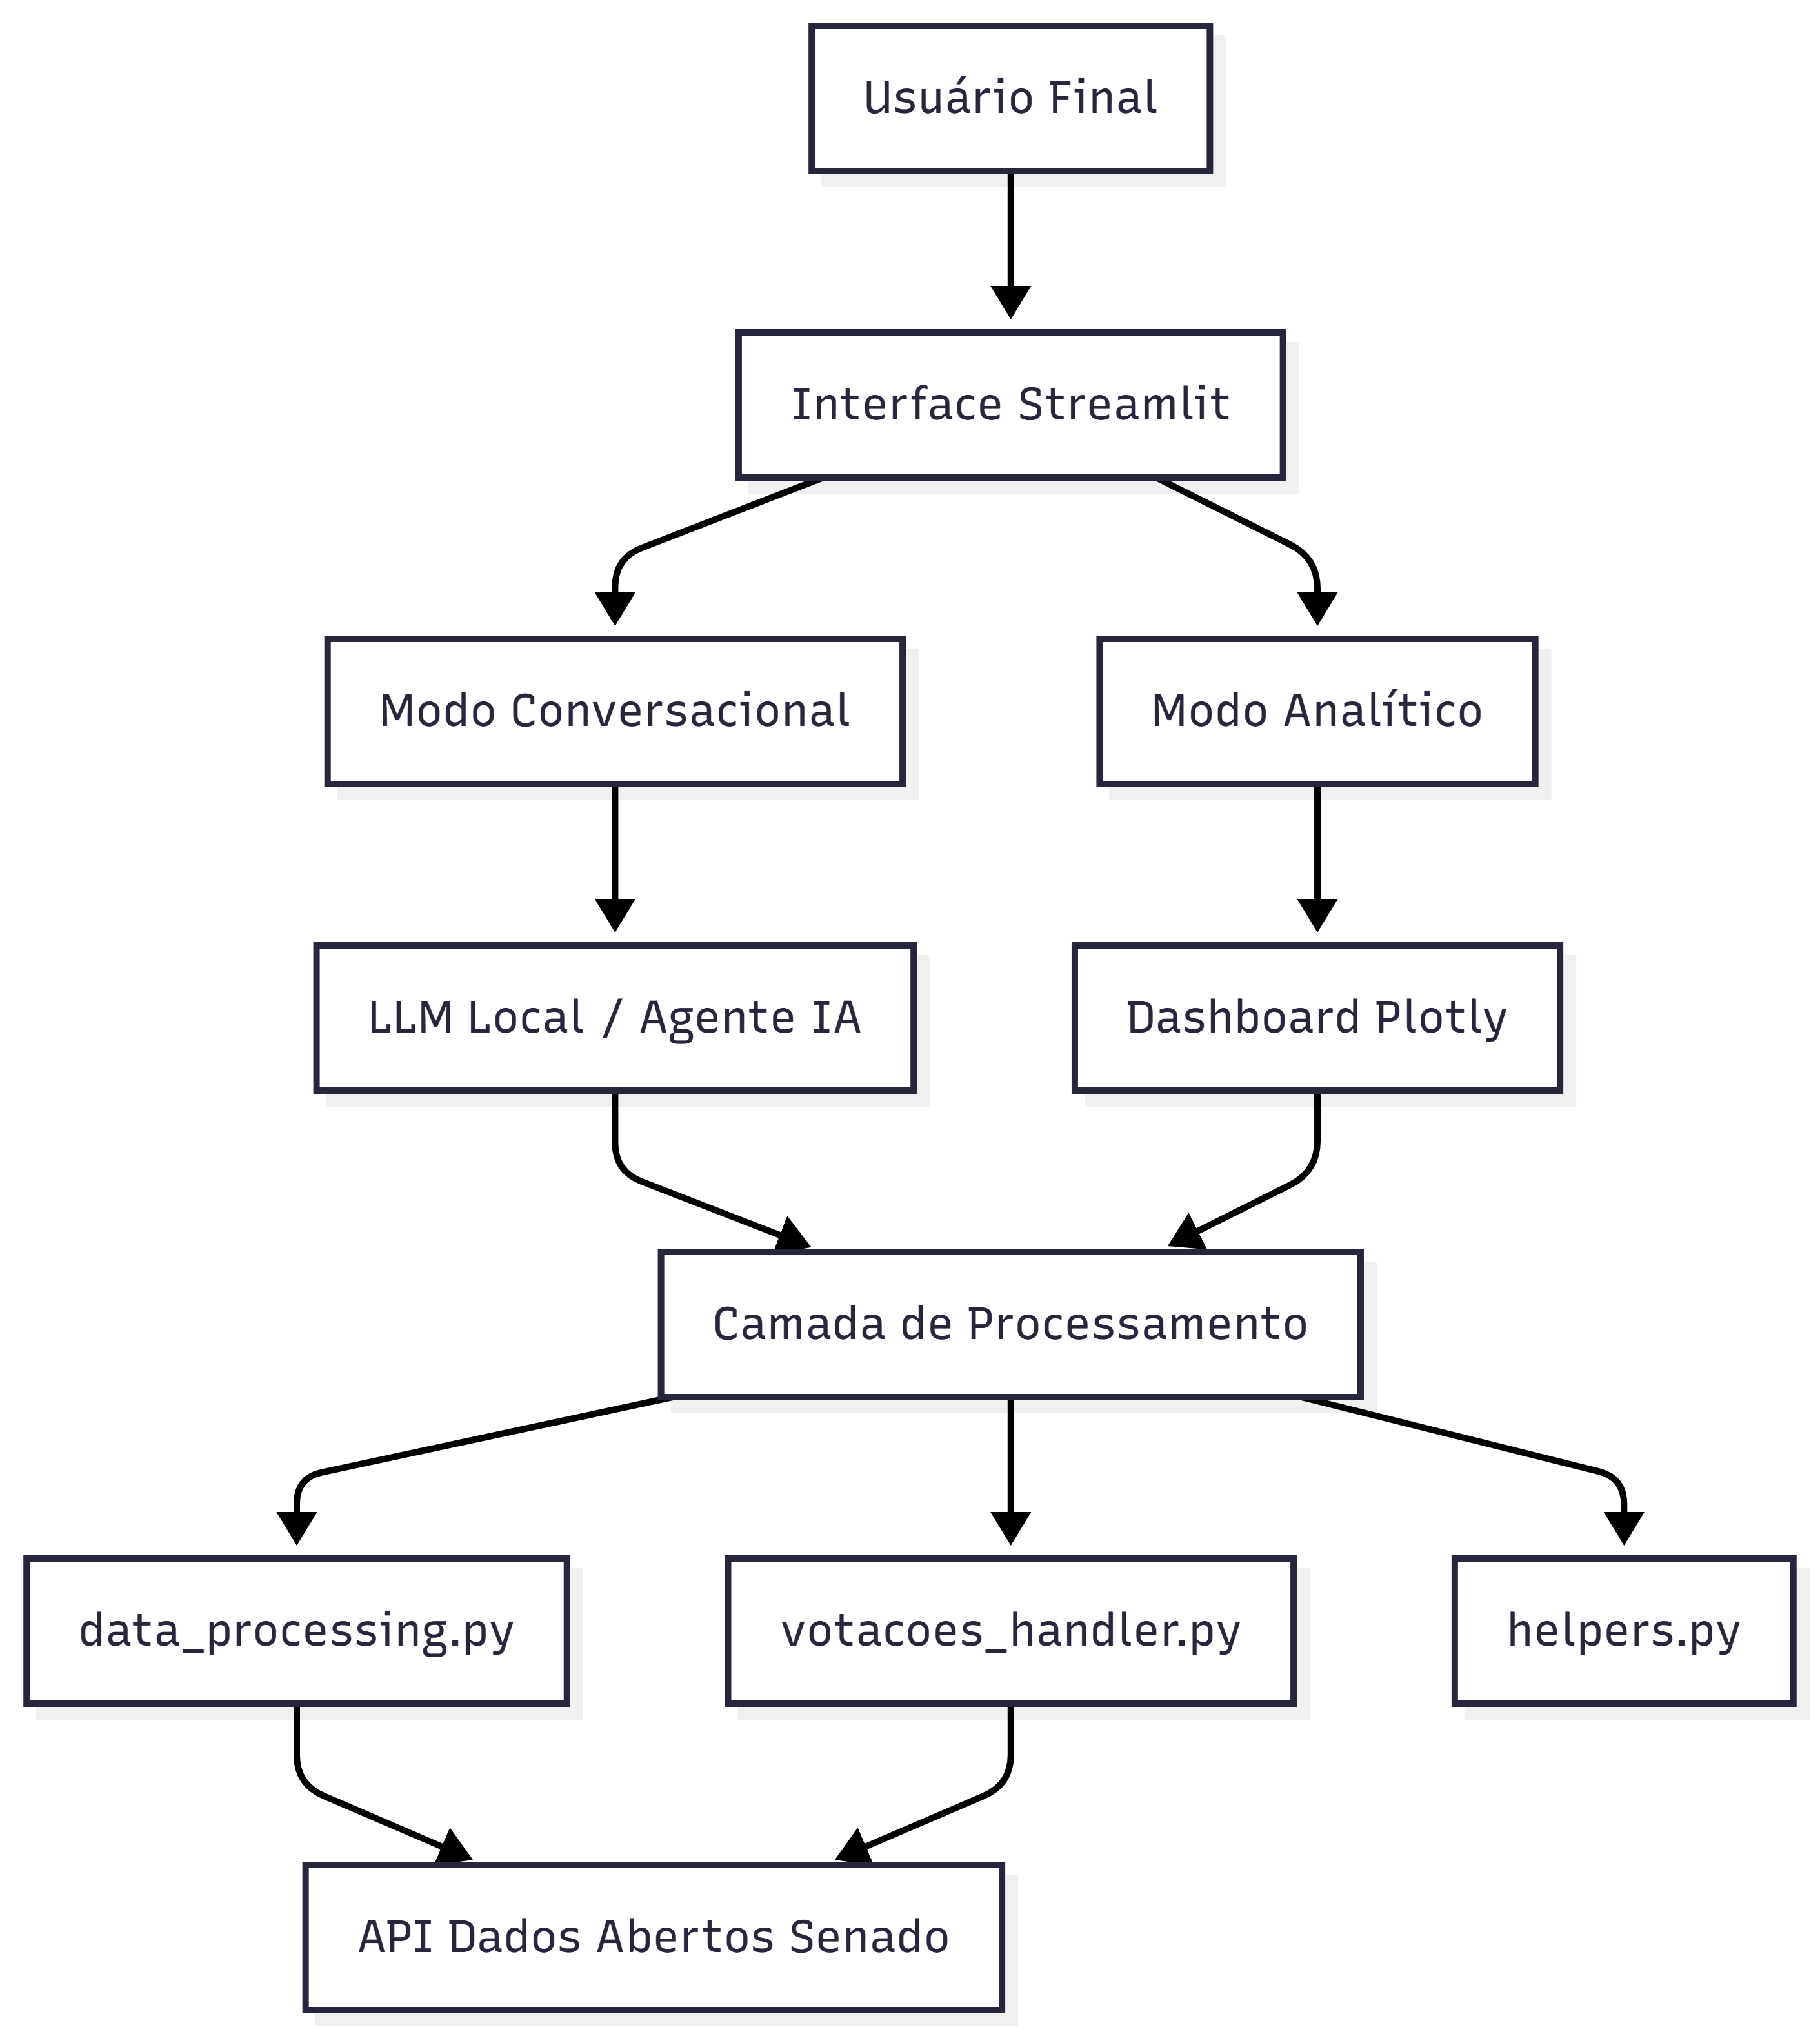
\includegraphics[width=0.9\textwidth]{imagens/arquitetura_aplicacao.png}
\fonte{Produção da autora.}
\end{figure}

Os conceitos discutidos neste capítulo não são independentes entre si: a teoria de dados abertos delimita o corpus e justifica a escolha da API do Senado Federal; os estudos sobre literacia de dados e barreiras cognitivas sustentam a decisão de oferecer duas modalidades de interação (visual e conversacional) em vez de apenas uma; o DSR fundamenta a abordagem metodológica que orienta todo o ciclo de pesquisa; e a discussão sobre RAG e alucinações em LLMs antecipa os desafios concretos que o protocolo de avaliação precisará endereçar. A articulação entre essas dimensões é o que diferencia a proposta de uma simples implementação técnica.

\chapter{Metodologia}
\label{cap:metodologia}
Quando o objetivo central de uma pesquisa é construir e avaliar um artefato computacional — e não apenas observar ou descrever um fenômeno —, a escolha metodológica deve refletir essa natureza construtiva. É nesse sentido que se adota o \textit{Design Science Research} (DSR), um paradigma consolidado em Ciência da Computação que orienta não apenas a construção do artefato, mas a geração de conhecimento científico a partir do processo de design, implementação e avaliação \cite{Peffers2007}. O risco de trabalhos dessa natureza é reduzir-se a um relatório técnico de desenvolvimento de software; a DSR evita isso ao exigir que cada decisão de design seja justificada teoricamente e que os resultados sejam avaliados com rigor comparável ao de pesquisas empíricas \cite{Runeson2020, Pimentel2020}. As seis fases que estruturam esta pesquisa são descritas a seguir.

\section{Abordagem Metodológica: Design Science Research}

A metodologia foi estruturada seguindo o ciclo de processo proposto por Peffers et al. \cite{Peffers2007}, adaptado para o contexto deste trabalho em seis fases principais, conforme ilustrado na Figura \ref{fig:fluxo_trabalho_projeto}:

\begin{enumerate}
    \item Identificação do Problema e Motivação
    \item Definição dos Objetivos da Solução
    \item Design e Desenvolvimento do Artefato
    \item Demonstração
    \item Avaliação
    \item Reflexão e Aprendizados
\end{enumerate}

\begin{figure}[H]
    \centering
    \caption{Fluxo metodológico baseado em Design Science Research (adaptado de Peffers et al. 2007)}
    \label{fig:fluxo_trabalho_projeto}
    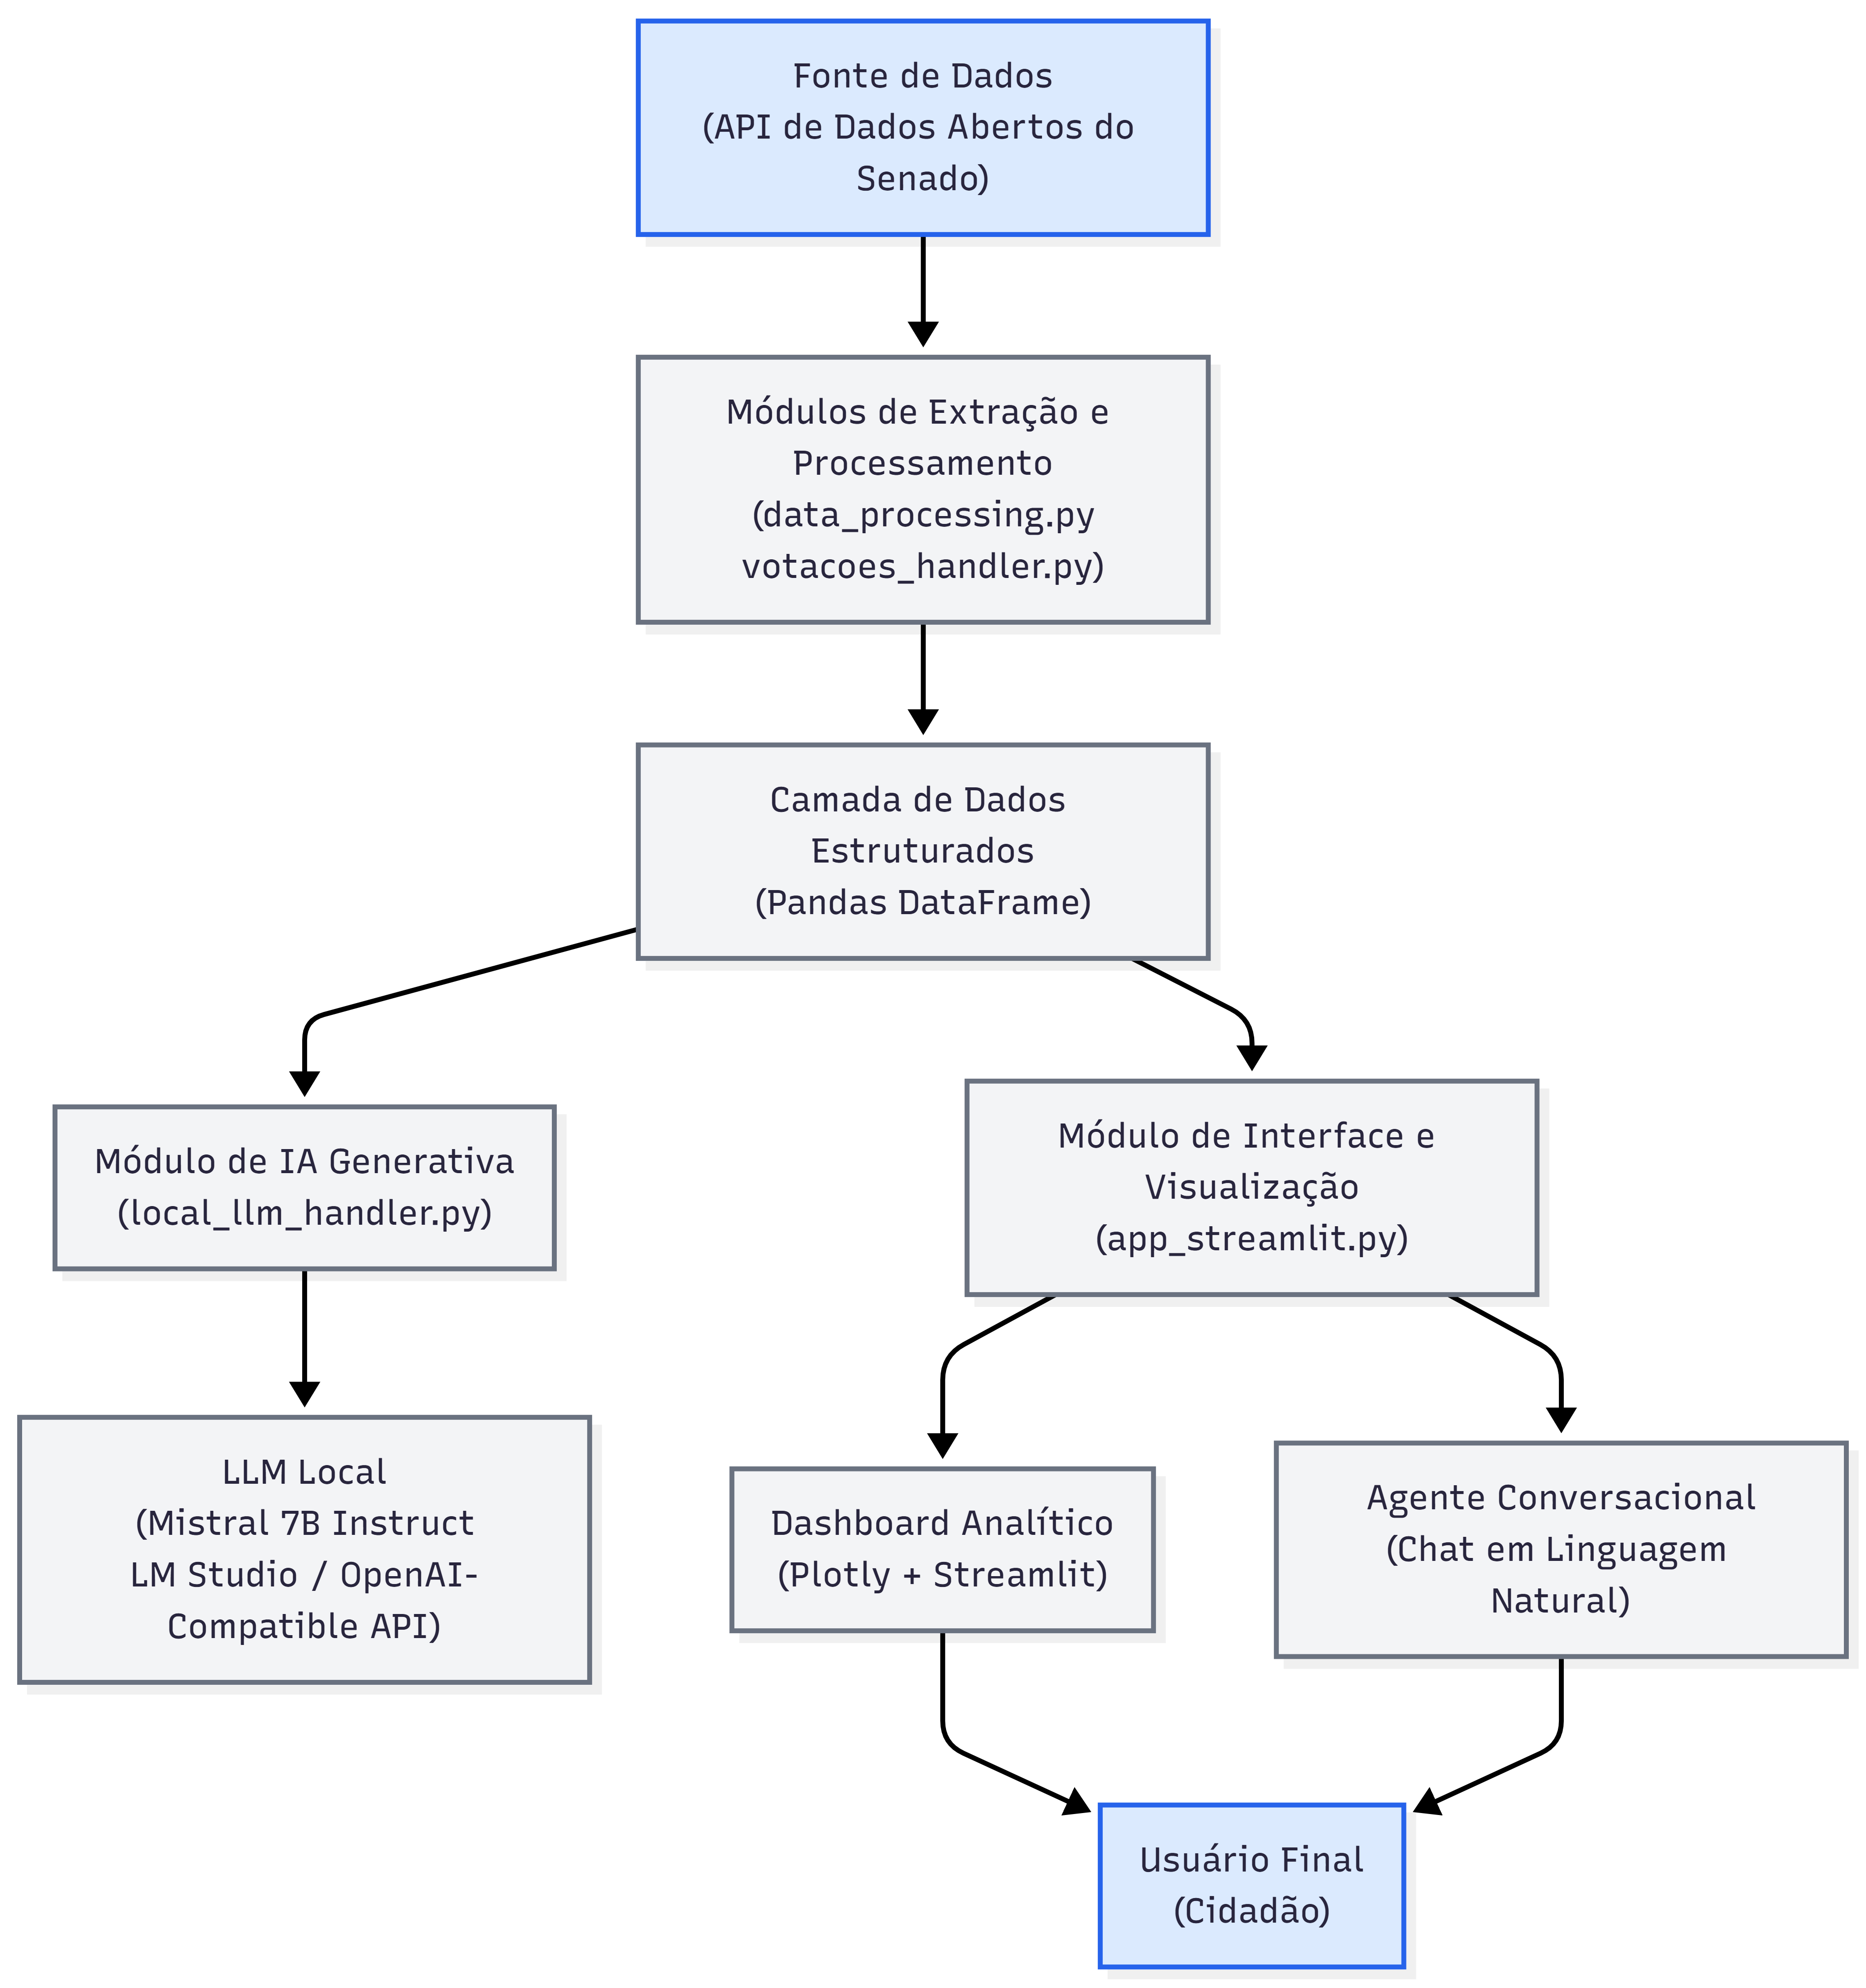
\includegraphics[width=0.8\textwidth]{imagens/fluxo_trabalho_projeto.png}
    \fonte{Adaptado de Peffers et al. (2007).}
\end{figure}

\section{Fases da Pesquisa}

\subsection{Fase 1: Identificação do Problema e Motivação}

A primeira etapa consistiu no reconhecimento da opacidade prática dos dados parlamentares. Embora disponíveis em formato aberto através da API do Senado Federal, a complexidade técnica e o volume massivo desses dados impedem que cidadãos comuns exerçam controle social efetivo. Segundo Oliveira e Ckagnazaroff \cite{OliveiraCkagnazaroff2022}, para que a transparência seja efetiva, os dados devem ser não apenas públicos, mas também claros, contextualizados e utilizáveis.

Conforme apontado por Lee et al. \cite{Lee2017} através do VLAT, nem todos conseguem interpretar visualizações gráficas complexas. Complementarmente, Hornung et al. \cite{Hornung2015} demonstram que usuários sem formação estatística frequentemente não conseguem analisar dados de forma autônoma. Consequentemente, a mera disponibilização de dados não garante compreensão ou participação democrática.

Esta fase foi fundamentada em revisão de literatura e análise exploratória da API do Senado Federal, identificando-se a lacuna entre disponibilidade técnica de dados e acessibilidade cognitiva para cidadãos.

\subsection{Fase 2: Definição dos Objetivos da Solução}

Definiu-se que o artefato a ser construído deveria reduzir as barreiras cognitivas de acesso aos dados parlamentares. Para isso, estabeleceu-se que a solução deveria:

\begin{enumerate}
    \item \textbf{Automatizar a extração de dados brutos:} Implementar pipeline de ETL para processar dados da API do Senado, convertendo formatos não estruturados (XML/JSON) em estruturas tabulares otimizadas para análise.

    \item \textbf{Traduzir linguagem parlamentar:} Utilizar IA Generativa para categorizar e resumir discursos parlamentares complexos, tornando-os compreensíveis para cidadãos sem expertise na área.

    \item \textbf{Permitir interação em linguagem natural:} Implementar interface conversacional que permita ao usuário formular perguntas em linguagem comum, dispensando conhecimento técnico de queries ou programação.

    \item \textbf{Oferecer múltiplas modalidades de exploração:} Combinar Dashboard visual (para exploração livre) com Chatbot conversacional (para consultas diretas), atendendo diferentes estilos cognitivos de usuários.
\end{enumerate}

\section{Fase 3: Design e Desenvolvimento do Artefato}

Nesta fase, correspondente à construção técnica da solução, a aplicação foi desenvolvida em Python sob uma arquitetura modular, visando garantir manutenibilidade e escalabilidade. A solução foi segmentada em três camadas principais:

\subsection{Coleta e Processamento de Dados (Camada de Dados)}

A coleta foi efetuada via API de Dados Abertos do Senado Federal \cite{SenadoFederal_s_d}. O processo de ETL (\textit{Extract, Transform, Load}) incluiu:

\begin{itemize}
    \item \textbf{Requisição:} Uso da biblioteca \textit{Requests} \cite{RequestsLib} para extração de dados brutos (XML/JSON) dos \textit{endpoints} mapeados via Swagger (Figura \ref{fig:senado_swagger}).
    \item \textbf{Estruturação:} Conversão e limpeza dos dados utilizando \textit{Pandas} \cite{PandasLib}, organizando discursos e votações em estruturas tabulares otimizadas para análise.
\end{itemize}

\begin{figure}[H]
    \centering
    \caption{Interface Swagger da API de Dados Abertos do Senado Federal}
    \label{fig:senado_swagger}
    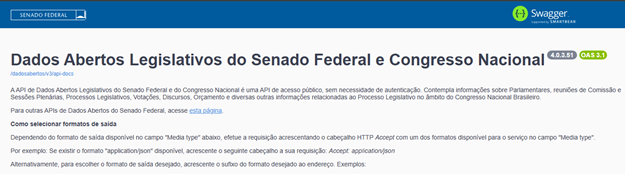
\includegraphics[width=0.9\textwidth]{imagens/senado_swagger.png}
    \fonte{Senado Federal.}
\end{figure}

\subsection{Análise com IA Generativa (Camada de Inteligência)}

O núcleo analítico utiliza o modelo Mistral 7B Instruct \cite{MistralAI2024}, que roda em ambiente local. Diferente de abordagens que dependem de APIs proprietárias, esta etapa emprega engenharia de \textit{prompts} para duas funções críticas:

\begin{itemize}
    \item \textbf{Classificação Temática:} Categorização automática de discursos em temas (ex: "Saúde", "Educação", "Infraestrutura") utilizando \textit{prompts} estruturados e exemplos de Few-Shot Learning.

    \item \textbf{Motor de Resposta (Recuperação Estruturada com Geração Aumentada):} O módulo recebe perguntas do usuário em linguagem natural, recupera da base em memória (cache de sessão) um subconjunto de registros relevantes e instrui o modelo Mistral 7B a gerar respostas contextualizadas e didáticas, compreensíveis para cidadãos não-especialistas, fundamentadas nesses registros e citando-os por identificador estável, de modo a preservar a rastreabilidade entre resposta e dados.
\end{itemize}

A justificativa detalhada para a escolha do Mistral 7B em ambiente local --- replicabilidade, soberania de dados e sustentabilidade operacional ---, bem como a comparação com modelos proprietários e com outros modelos abertos contemporâneos, encontra-se na fundamentação teórica (Seção~\ref{subsec:escolha_modelo}). Aqui interessa registrar apenas que essa decisão de design condiciona o protocolo de avaliação descrito adiante, em especial a comparação da classificação temática com uma linha de base sem LLM.

\subsection{Interface Interativa (Camada de Apresentação)}

Para materializar o acesso democrático aos dados, desenvolveu-se uma interface \textit{web} utilizando o \textit{framework Streamlit} \cite{Streamlit2024}, oferecendo dois modos de interação complementares:

\begin{itemize}
    \item \textbf{\textit{Dashboard} Visual:} Gráficos interativos gerados com \textit{Plotly} \cite{Plotly2024} para exploração de tendências legislativas. O dashboard permite que usuários visualizem panoramicamente os dados, seguindo o princípio de Shneiderman \cite{Shneiderman1996} de "zoom and filter" (Figura \ref{fig:tela_aplicacao}).

    \item \textbf{Agente Conversacional:} Interface de \textit{chat} que abstrai a complexidade dos dados, permitindo consultas diretas em linguagem natural como "Como votou o Senador X sobre educação?" ou "Qual foi o tema mais debatido em 2025?" (Figura \ref{fig:tela_aplicacao}).
\end{itemize}

\begin{figure}[H]
    \centering
    \caption{Interface da Aplicação}
    \label{fig:tela_aplicacao}
    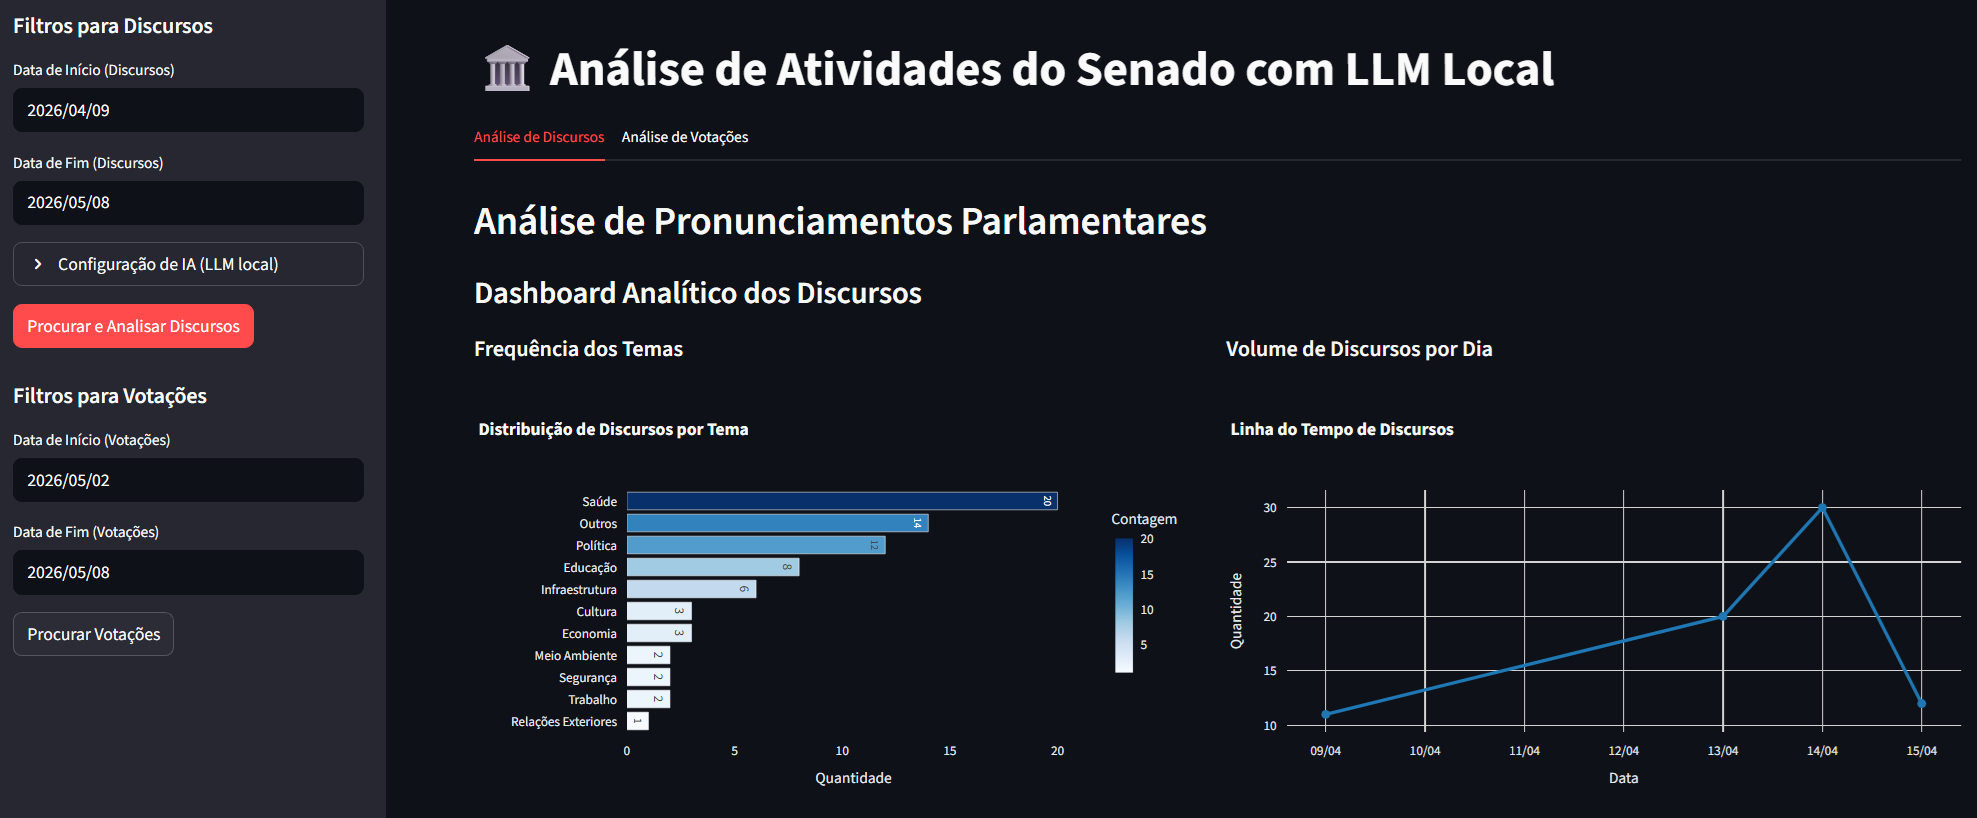
\includegraphics[width=0.9\textwidth]{imagens/tela_aplicacao.png}
    \fonte{Produção da autora.}
\end{figure}

\section{Fundamentos Teóricos para as Escolhas de Design}

A combinação de Dashboard e Chatbot não é arbitrária, mas fundamentada em teorias de Interação Humano-Computador e Acessibilidade de Dados. Esta seção justifica essas escolhas.

\subsection{Por que Dashboard?}

Dashboards e visualizações de dados oferecem exploração livre e visão holística de um corpus de dados. Contudo, conforme Lee et al. \cite{Lee2017} demonstram através do VLAT, nem todos os usuários possuem "visualization literacy" — a capacidade de compreender visualizações gráficas complexas.

Apesar dessa limitação, os \textit{dashboards} oferecem benefícios concretos: permitem ao usuário obter uma visão panorâmica dos dados antes de descer ao detalhe --- seguindo o princípio de Shneiderman \cite{Shneiderman1996} ---, explorar o corpus de forma autônoma e sem intermediário, identificar padrões visuais como tendências e anomalias e, ainda, filtrar e segmentar a informação interativamente. Por isso, o \textit{dashboard} proposto adota decisões de design voltadas à acessibilidade: paleta de cores intuitiva, títulos e rótulos em linguagem comum em vez de jargão legislativo, preferência por representações simples --- barras e linhas --- em detrimento de \textit{heatmaps} ou \textit{scatter plots}, e interatividade básica baseada em filtros e em detalhamento sob demanda.

\subsection{Por que Chatbot?}

Interfaces conversacionais, especialmente aquelas alimentadas por Modelos de Linguagem Generativa, reduzem significativamente a barreira de entrada cognitiva. Um usuário sem expertise estatística pode formular perguntas em linguagem natural em vez de construir queries SQL ou manipular dados brutos.

Conforme a pesquisa em Interação Humano-Computador e Interação Humano-Dados \cite{Hornung2015, Brito2024}, as interfaces conversacionais reduzem a barreira de entrada --- o usuário não precisa conhecer a estrutura dos dados nem uma linguagem de consulta ---, apoiam-se em um formato de interação familiar, acomodam formulações distintas para uma mesma necessidade de informação e podem mediar a compreensão, traduzindo resultados técnicos em explicações acessíveis.

Essas vantagens convivem com limitações conhecidas dos \textit{chatbots} baseados em LLMs, sobretudo o risco de alucinação (respostas factualmente incorretas) e a opacidade do processo de geração. Para mitigá-las, a implementação proposta utiliza o Mistral 7B Instruct \cite{Jiang2023}, cujo porte paramétrico reduz a incidência de alucinações em relação a modelos de menor escala; valida as respostas contra os dados reais; e --- ponto central deste trabalho --- garante rastreabilidade, pois o agente recupera um subconjunto de registros da base, cita-os na resposta por identificador estável e expõe, na interface, o painel de fontes utilizadas.

\subsection{Complementaridade: Dashboard + Chatbot}

A literatura em Interação Humano-Dados distingue dois padrões primários de uso em sistemas de informação pública: a exploração orientada à descoberta, em que o usuário navega pelo corpus sem uma pergunta pré-definida, e a consulta orientada a objetivos, em que há uma pergunta específica a ser respondida \cite{Shneiderman1996}. Esses padrões raramente são atendidos com igual eficácia por uma única modalidade de interface.

O \textit{Dashboard} atende principalmente o primeiro padrão: permite ao usuário identificar tendências, comparar parlamentares e detectar anomalias por navegação visual, sem exigir que ele formule uma pergunta antes de começar. O \textit{Chatbot}, por sua vez, é mais adequado ao segundo padrão: reduz a carga cognitiva de quem sabe o que quer perguntar mas não sabe como navegar em dados estruturados. A integração de ambos em um único sistema não busca cobrir todos os perfis de usuário possíveis — uma afirmação que exigiria validação empírica — mas reconhece que restringir a interação a uma única modalidade excluiria sistematicamente parte dos potenciais usuários. Essa decisão de design será discutida nas considerações finais à luz dos resultados da avaliação.

\section{Fase 4: Demonstração}

Em DSR, a Demonstração distingue-se da Avaliação: enquanto esta confronta o artefato com critérios pré-definidos, aquela evidencia a viabilidade do artefato em uso, por meio de ao menos um cenário representativo documentado de ponta a ponta. Nesta fase, o AgentAI foi colocado em ambiente de homologação, processando dados reais da API do Senado Federal, e sua operação foi demonstrada em um fluxo completo: a partir de uma pergunta em linguagem natural (entrada), o sistema recupera os registros pertinentes da base (processamento), gera uma resposta fundamentada (saída) e exibe os registros que a embasam (fontes). Esse fluxo abrange o processamento automático de sessões legislativas reais, a classificação temática dos discursos, a resposta a consultas em linguagem natural e a visualização de tendências legislativas, confirmando a viabilidade técnica que habilita a fase de avaliação rigorosa. A verificação funcional preliminar correspondente é reportada no Capítulo~\ref{cap:desenvolvimento}.

\section{Fase 5: Avaliação do Artefato}

A fase de avaliação será conduzida sem entrevistas, questionários, observação comportamental ou qualquer coleta de dados com participantes humanos. A avaliação incidirá sobre o artefato computacional, os dados públicos processados e as respostas geradas pelo modelo. Dessa forma, a pesquisa utiliza exclusivamente dados abertos, informações de domínio público e análises técnicas do sistema.

A avaliação foi organizada em quatro frentes complementares: qualidade da coleta e estruturação dos dados, classificação temática, qualidade factual das respostas e rastreabilidade das informações apresentadas pelo agente conversacional. O Quadro~\ref{quad:matriz_rastreabilidade} explicita o alinhamento entre os objetivos específicos, as frentes de avaliação, as métricas e as cláusulas da hipótese, tornando rastreável a cadeia que liga a questão de pesquisa aos critérios de avaliação.

\begin{quadro}[H]
    \centering
    \caption{Matriz de rastreabilidade entre objetivos, frentes de avaliação, métricas e cláusulas da hipótese}
    \label{quad:matriz_rastreabilidade}
    \resizebox{\textwidth}{!}{%
    \begin{tabular}{|p{4.2cm}|p{3.4cm}|p{5.0cm}|p{2.4cm}|}
        \hline
        \textbf{Objetivo específico} & \textbf{Frente de avaliação} & \textbf{Métricas principais} & \textbf{Cláusula da hipótese} \\
        \hline
        Processar e estruturar os dados da API do Senado & Coleta e estruturação & Completude, consistência, reprodutibilidade & Premissa (estruturar) \\
        \hline
        Classificar tematicamente os discursos & Classificação temática & Acurácia, precisão, revocação e F1 \textit{vs.} \textit{baseline} sem LLM & (a) \\
        \hline
        Responder em linguagem natural sobre os dados & Avaliação factual & \% de respostas corretas/parciais/incorretas \textit{vs.} configuração sem recuperação & (b) \\
        \hline
        Avaliar a rastreabilidade das respostas & Rastreabilidade & Cobertura de recuperação e de citação, precisão e suporte semântico da citação & (c) \\
        \hline
        Consolidar o uso do artefato & Cenários de uso & Síntese qualitativa dos casos de teste & Premissa (consultar) \\
        \hline
    \end{tabular}%
    }
    \fonte{Produção da autora.}
\end{quadro}

\subsection{Avaliação da Coleta e Estruturação dos Dados}

\subsubsection{Pergunta}
Em que medida o pipeline de coleta e processamento estrutura corretamente os dados parlamentares obtidos da API do Senado Federal?

\subsubsection{Método}
Será selecionado um conjunto de endpoints e períodos de coleta definidos no escopo do estudo. Os dados retornados pela API serão comparados com as estruturas armazenadas localmente pelo AgentAI, verificando se os campos essenciais foram preservados e se o processo de transformação não introduziu inconsistências.

\subsubsection{Métricas}
\begin{itemize}
    \item \textbf{Completude:} proporção de registros coletados e armazenados com campos essenciais preenchidos.
    \item \textbf{Consistência:} ausência de duplicidades, datas inválidas, campos incompatíveis ou vínculos incorretos entre parlamentar, discurso, votação e matéria.
    \item \textbf{Reprodutibilidade:} capacidade de reexecutar o pipeline e obter uma base equivalente para o mesmo recorte temporal.
\end{itemize}

\subsection{Avaliação da Classificação Temática}

\subsubsection{Pergunta}
Em que medida o modelo Mistral 7B Instruct classifica corretamente os temas dos discursos parlamentares?

\subsubsection{Método}
As categorias temáticas serão definidas \textit{a priori}, antes de qualquer anotação, a partir das áreas recorrentes na atividade legislativa, fixando-se um número mínimo de instâncias por categoria (ao menos 20) para assegurar a estabilidade das métricas por classe. Sobre essa base, será construída uma amostra de discursos reais do Senado Federal (mínimo de 150 registros, distribuídos entre as categorias) para compor o gabarito de referência. A anotação será realizada de forma independente por dois avaliadores, guiada por um protocolo documentado explicitamente antes do início --- com a definição operacional de cada categoria e exemplos de casos limítrofes. O nível de concordância entre os avaliadores será medido pelo coeficiente Kappa de Cohen \cite{Cohen1960}, adotando-se, antes da anotação, o limiar de concordância substancial ($\kappa \geq 0{,}61$) da escala de Landis e Koch \cite{LandisKoch1977} como critério mínimo aceitável; abaixo desse valor, o protocolo será revisado e a anotação refeita. Para reduzir o risco de viés compartilhado, os casos de discordância remanescentes serão resolvidos por um terceiro anotador independente, e não por discussão entre os dois anotadores iniciais; a concordância será reportada também por classe. A classificação gerada pelo modelo será então comparada com o gabarito final.

\subsubsection{Métricas}
\begin{itemize}
    \item \textbf{Acurácia:} proporção de classificações coincidentes com o gabarito de referência.
    \item \textbf{Precisão:} proporção de discursos classificados em um tema que efetivamente pertencem a esse tema no gabarito.
    \item \textbf{Revocação:} proporção de discursos de um tema que foram corretamente identificados pelo modelo.
    \item \textbf{F1-Score:} média harmônica entre precisão e revocação.
\end{itemize}

\subsubsection{Critério de Interpretação}
Os resultados serão interpretados comparativamente em relação a um \textit{baseline} de referência: uma classificação por correspondência de palavras-chave temáticas predefinidas (abordagem clássica sem LLM). Essa comparação permite dimensionar o ganho — ou ausência de ganho — que o Mistral 7B Instruct oferece em relação a uma solução mais simples. A análise qualitativa complementará os números, identificando os tipos de discurso que geram maior ambiguidade e os casos em que o modelo produz classificações inconsistentes com o gabarito.

\subsection{Avaliação Factual das Respostas do Agente Conversacional}

\subsubsection{Pergunta}
As respostas geradas pelo agente conversacional são coerentes com os dados públicos recuperados da base local?

\subsubsection{Método}
Será elaborado um conjunto de cenários representativos de consulta, definido \textit{a priori} e dimensionado para cobrir todas as classes de pergunta previstas (votações, discursos, parlamentares, temas e períodos) com múltiplas instâncias por classe, totalizando ao menos 30 cenários. Para cada cenário, será definida uma resposta esperada com base nos dados oficiais coletados da API do Senado Federal. As respostas geradas pelo AgentAI serão classificadas em quatro categorias com definição operacional explícita: \textit{correta} (todas as afirmações verificáveis conferem com os dados e nada essencial é omitido); \textit{parcialmente correta} (afirmações corretas convivem com omissões ou imprecisões não centrais); \textit{incorreta} (há ao menos uma afirmação factualmente errada ou sem respaldo nos dados); e \textit{não respondida} (o sistema não responde ou declara não dispor da informação). Para reduzir a subjetividade, a classificação será conduzida por dois avaliadores de forma independente, com a concordância medida pelo Kappa de Cohen \cite{Cohen1960} e as divergências resolvidas por um terceiro avaliador; sempre que a comparação envolver as configurações com e sem recuperação contextual, o avaliador será cegado quanto à origem da resposta. O protocolo será fixado antes da execução.

\subsubsection{Métricas}
\begin{itemize}
    \item Percentual de respostas corretas.
    \item Percentual de respostas parcialmente corretas.
    \item Percentual de respostas incorretas ou sem respaldo nos dados.
    \item Tipos de erro observados, como omissão, generalização indevida, interpretação incorreta ou ausência de evidência recuperada.
\end{itemize}

\subsection{Avaliação de Rastreabilidade}

\subsubsection{Pergunta}
As respostas do agente conversacional permitem identificar os dados utilizados para sua geração?

\subsubsection{Método}
O artefato já implementa rastreabilidade em dois níveis --- na resposta ao usuário e na instrumentação de medição (Capítulo~\ref{cap:desenvolvimento}). A avaliação apoia-se nessa instrumentação: cada consulta é registrada em \textit{log} estruturado (\texttt{qa\_trace.jsonl}) contendo a pergunta, os identificadores das fontes recuperadas e a resposta gerada, e um módulo de avaliação processa esse registro para quantificar o vínculo entre resposta e dados. Sobre o mesmo conjunto de cenários da avaliação factual, a análise verificará se a resposta cita as fontes efetivamente recuperadas e se evita referenciar dados fora do contexto recuperado. Além da verificação do vínculo formal --- a existência do identificador entre as fontes ---, o protocolo incorpora a verificação de \textbf{suporte semântico} da citação, isto é, se o registro citado de fato sustenta a afirmação a que está associado, combinando uma checagem automática de sobreposição entre os termos da afirmação e o conteúdo da fonte com a anotação manual de uma amostra. A instrumentação encontra-se pronta e validada de ponta a ponta; o que constitui a etapa em execução desta fase é a medição sobre o conjunto de cenários definido.

\subsubsection{Métricas}
\begin{itemize}
    \item \textbf{Cobertura de recuperação:} proporção de consultas para as quais o sistema recupera ao menos um registro da base como fonte da resposta.
    \item \textbf{Cobertura de citação:} proporção de respostas que citam explicitamente, por identificador, ao menos uma das fontes recuperadas.
    \item \textbf{Precisão de citação:} proporção de identificadores citados nas respostas que de fato correspondem a registros presentes no conjunto de fontes recuperado.
    \item \textbf{Suporte semântico da citação:} proporção de citações em que a fonte referenciada efetivamente sustenta a afirmação a que está associada, verificada automaticamente por sobreposição de termos e confirmada por anotação manual em uma amostra.
\end{itemize}

\subsubsection{Limitações Assumidas}
A noção \textit{formal} de rastreabilidade --- a mera existência do identificador citado entre as fontes --- é insuficiente, pois uma resposta poderia citar um registro que não sustenta a afirmação. Por isso, conforme descrito no método, esta avaliação não se limita ao vínculo formal: incorpora a verificação de suporte semântico da citação, o que torna a cláusula (c) da hipótese efetivamente testável. Permanecem como limitações assumidas: (i) perguntas de natureza agregada (por exemplo, ``quantos senadores discursaram sobre saúde?'') podem ser respondidas corretamente sem citar uma fonte específica, razão pela qual a cobertura de citação será reportada de forma segmentada por tipo de pergunta; e (ii) a verificação automática de suporte semântico, baseada em sobreposição lexical, é aproximada, sendo por isso complementada pela anotação manual de uma amostra.

\subsection{Avaliação de Cenários de Uso}

A avaliação final consolidará os resultados das etapas anteriores em cenários de uso definidos pela pesquisadora. Esses cenários não envolvem participantes externos; funcionam como casos de teste do artefato. Exemplos incluem: consultar o posicionamento de um parlamentar em uma votação, identificar temas recorrentes em discursos de um período e solicitar uma síntese de votações relacionadas a uma área temática.
\section{Fase 6: Reflexão e Aprendizados}

A fase final documenta o conhecimento científico gerado através da pesquisa. Não se trata apenas de documentar que o artefato funciona tecnicamente, mas de analisar sistematicamente:

\begin{itemize}
    \item O que aprendemos sobre design de interfaces para acessibilidade de dados?
    \item Que padrões emergiram dos cenários de avaliação técnica?
    \item Quais são as limitações da abordagem com IA Generativa?
    \item Que contribuições esta pesquisa oferece para a comunidade científica?
\end{itemize}

\section{Ameaças à Validade}

A avaliação proposta está sujeita a ameaças à validade que, seguindo a categorização clássica adotada na pesquisa empírica em Engenharia de Software \cite{Runeson2020}, organizam-se em quatro dimensões. Explicitá-las é condição para interpretar corretamente os resultados.

\subsection{Validade de Construto}
Refere-se a se as métricas medem aquilo que afirmam medir. A principal ameaça está na rastreabilidade: uma métrica puramente formal --- a existência do identificador citado --- não captura se a fonte sustenta a afirmação. Essa ameaça é mitigada pela métrica de suporte semântico e pela anotação manual de uma amostra. Ademais, a cobertura de recuperação tende a 100\% por construção, pois o mecanismo sempre retorna algum registro; por isso ela é interpretada como verificação de funcionamento, e não como evidência de qualidade.

\subsection{Validade Interna}
Diz respeito a fatores que podem distorcer a relação entre o artefato e os resultados observados. O principal risco é o viés de anotação --- critérios subjetivos na construção dos gabaritos e eventual não-independência entre anotadores. Mitiga-se com protocolo de anotação definido \textit{a priori}, dupla anotação independente, limiar de Kappa pré-fixado, terceiro anotador para desempate e cegamento do avaliador quanto à origem da resposta nas comparações com a linha de base.

\subsection{Validade Externa}
Refere-se à generalização dos resultados. O corpus restringe-se ao Senado Federal e ao recorte temporal de 2024 a 2026, de modo que os achados podem não se transferir para outras casas legislativas, períodos ou idiomas; do mesmo modo, conclusões obtidas com o Mistral 7B Instruct não se estendem automaticamente a outros modelos. Essas fronteiras são declaradas, e a arquitetura modular do artefato é apontada como caminho para replicação em outros contextos.

\subsection{Validade de Conclusão}
Relaciona-se à solidez das inferências. Como a avaliação se baseia em um conjunto finito de cenários definidos pela pesquisadora, sem participantes humanos, evita-se afirmar significância estatística: os resultados são reportados de forma descritiva e caracterizadora, com o número de cenários e de instâncias por classe declarados e comparados a \textit{baselines}. Limitações de tamanho de amostra são tratadas como restrição assumida, e não como achado conclusivo.

\section{Cronograma de Execução}

O planejamento para o período que se estende até a defesa, prevista para janeiro de 2027, foca na execução das Fases 5 e 6 (Avaliação e Reflexão) e na produção textual. O Quadro \ref{quad:cronograma_metodologia} detalha as atividades previstas até a defesa final.

\begin{quadro}[H]
    \centering
    \caption{Cronograma de Execução e Finalização da Dissertação}
    \label{quad:cronograma_metodologia}
    \resizebox{\textwidth}{!}{%
    \begin{tabular}{|p{8cm}|>{\centering\arraybackslash}p{2cm}|>{\centering\arraybackslash}p{2cm}|>{\centering\arraybackslash}p{2cm}|>{\centering\arraybackslash}p{2cm}|}
        \hline
        \textbf{Atividades (Fase Final)} & \textbf{Trim. 1 2026} & \textbf{Trim. 2 2026} & \textbf{Trim. 3 2026} & \textbf{Trim. 4 2026} \\
        \hline
        Ajustes pós-Qualificação (Metodologia DSR) & X & & & \\
        \hline
        Preparação do Gabarito Ouro (Classificação Manual) & X & X & & \\
        \hline
        Execução do Experimento de Acurácia (IA) & X & X & & \\
        \hline
        Avaliação factual das respostas geradas & & X & X & \\
        \hline
        Avaliação de rastreabilidade e cenários de consulta & & X & X & \\
        \hline
        Análise Estatística e Qualitativa dos Resultados & & X & X & \\
        \hline
        Artigo Científico: PROPOR 2026 (retorno negativo, fev/2026); ERBASE 2026 (submetido) & X & X & & \\
        \hline
        Escrita Final da Dissertação (Resultados + Conclusão) & & & X & X \\
        \hline
        Revisão e Depósito & & & & X \\
        \hline
        Defesa da Dissertação & & & & X \\
        \hline
    \end{tabular}%
    }
    \fonte{Produção da autora.}
\end{quadro}

As atividades estão distribuídas da seguinte forma:

\begin{itemize}
    \item \textbf{1º Trimestre 2026:} Refinamento do texto da proposta conforme feedback da banca, implementação de melhorias metodológicas, preparação do dataset de controle (Gabarito Ouro) para experimento de acurácia.

    \item \textbf{2º Trimestre 2026:} Execução dos testes técnicos para validação de acurácia, avaliação factual das respostas, verificação de rastreabilidade e execução de cenários representativos de consulta. Registra-se que um artigo científico foi submetido ao PROPOR 2026, tendo recebido retorno negativo em fevereiro de 2026; o trabalho foi revisado e submetido ao ERBASE 2026.

    \item \textbf{3º Trimestre 2026:} Consolidação estatística e qualitativa dos dados obtidos na avaliação, redação dos capítulos finais da dissertação (Análise de Resultados e Conclusão), finalização e submissão do artigo científico.

    \item \textbf{4º Trimestre 2026:} Revisão final do texto completo da dissertação, submissão para a banca examinadora, defesa pública.
\end{itemize}


\chapter{Estado da Arte}
\label{cap:estado_arte}
Este capítulo mapeia sistematicamente as pesquisas existentes na interseção entre Inteligência Artificial e dados parlamentares, com o objetivo de identificar o que já foi feito, onde estão as lacunas, e como este trabalho se posiciona em relação à literatura.

Optou-se pelo Mapeamento Sistemático da Literatura (MSL) em vez de uma revisão narrativa porque o escopo do tema é amplo e interdisciplinar — abrangendo PLN, dados abertos, transparência governamental e interação humano-dados —, o que exige um protocolo estruturado para evitar seleção tendenciosa de fontes \cite{Kitchenham2004}. A diferença entre MSL e revisão sistemática é relevante aqui: enquanto a revisão sistemática busca sintetizar evidências sobre uma intervenção específica, o mapeamento tem por objetivo caracterizar o espaço de pesquisa, identificar tendências e delimitar lacunas, o que é mais adequado para áreas emergentes como a aplicação de IA Generativa em contextos legislativos \cite{Kitchenham2004}.

O protocolo seguiu as diretrizes de Kitchenham \cite{Kitchenham2004}, estruturado em três fases: Planejamento, Execução e Análise.

\section{Protocolo do Mapeamento Sistemático}

O processo adotado seguiu as três fases críticas recomendadas pela literatura: Planejamento, Execução e Análise. Tal abordagem estruturada assegura o rigor na seleção dos estudos. A Figura \ref{fig:fase_rsl} ilustra o fluxo de trabalho.

\begin{figure}[H]
    \centering
    \caption{Fases do Mapeamento Sistemático da Literatura}
    \label{fig:fase_rsl}
    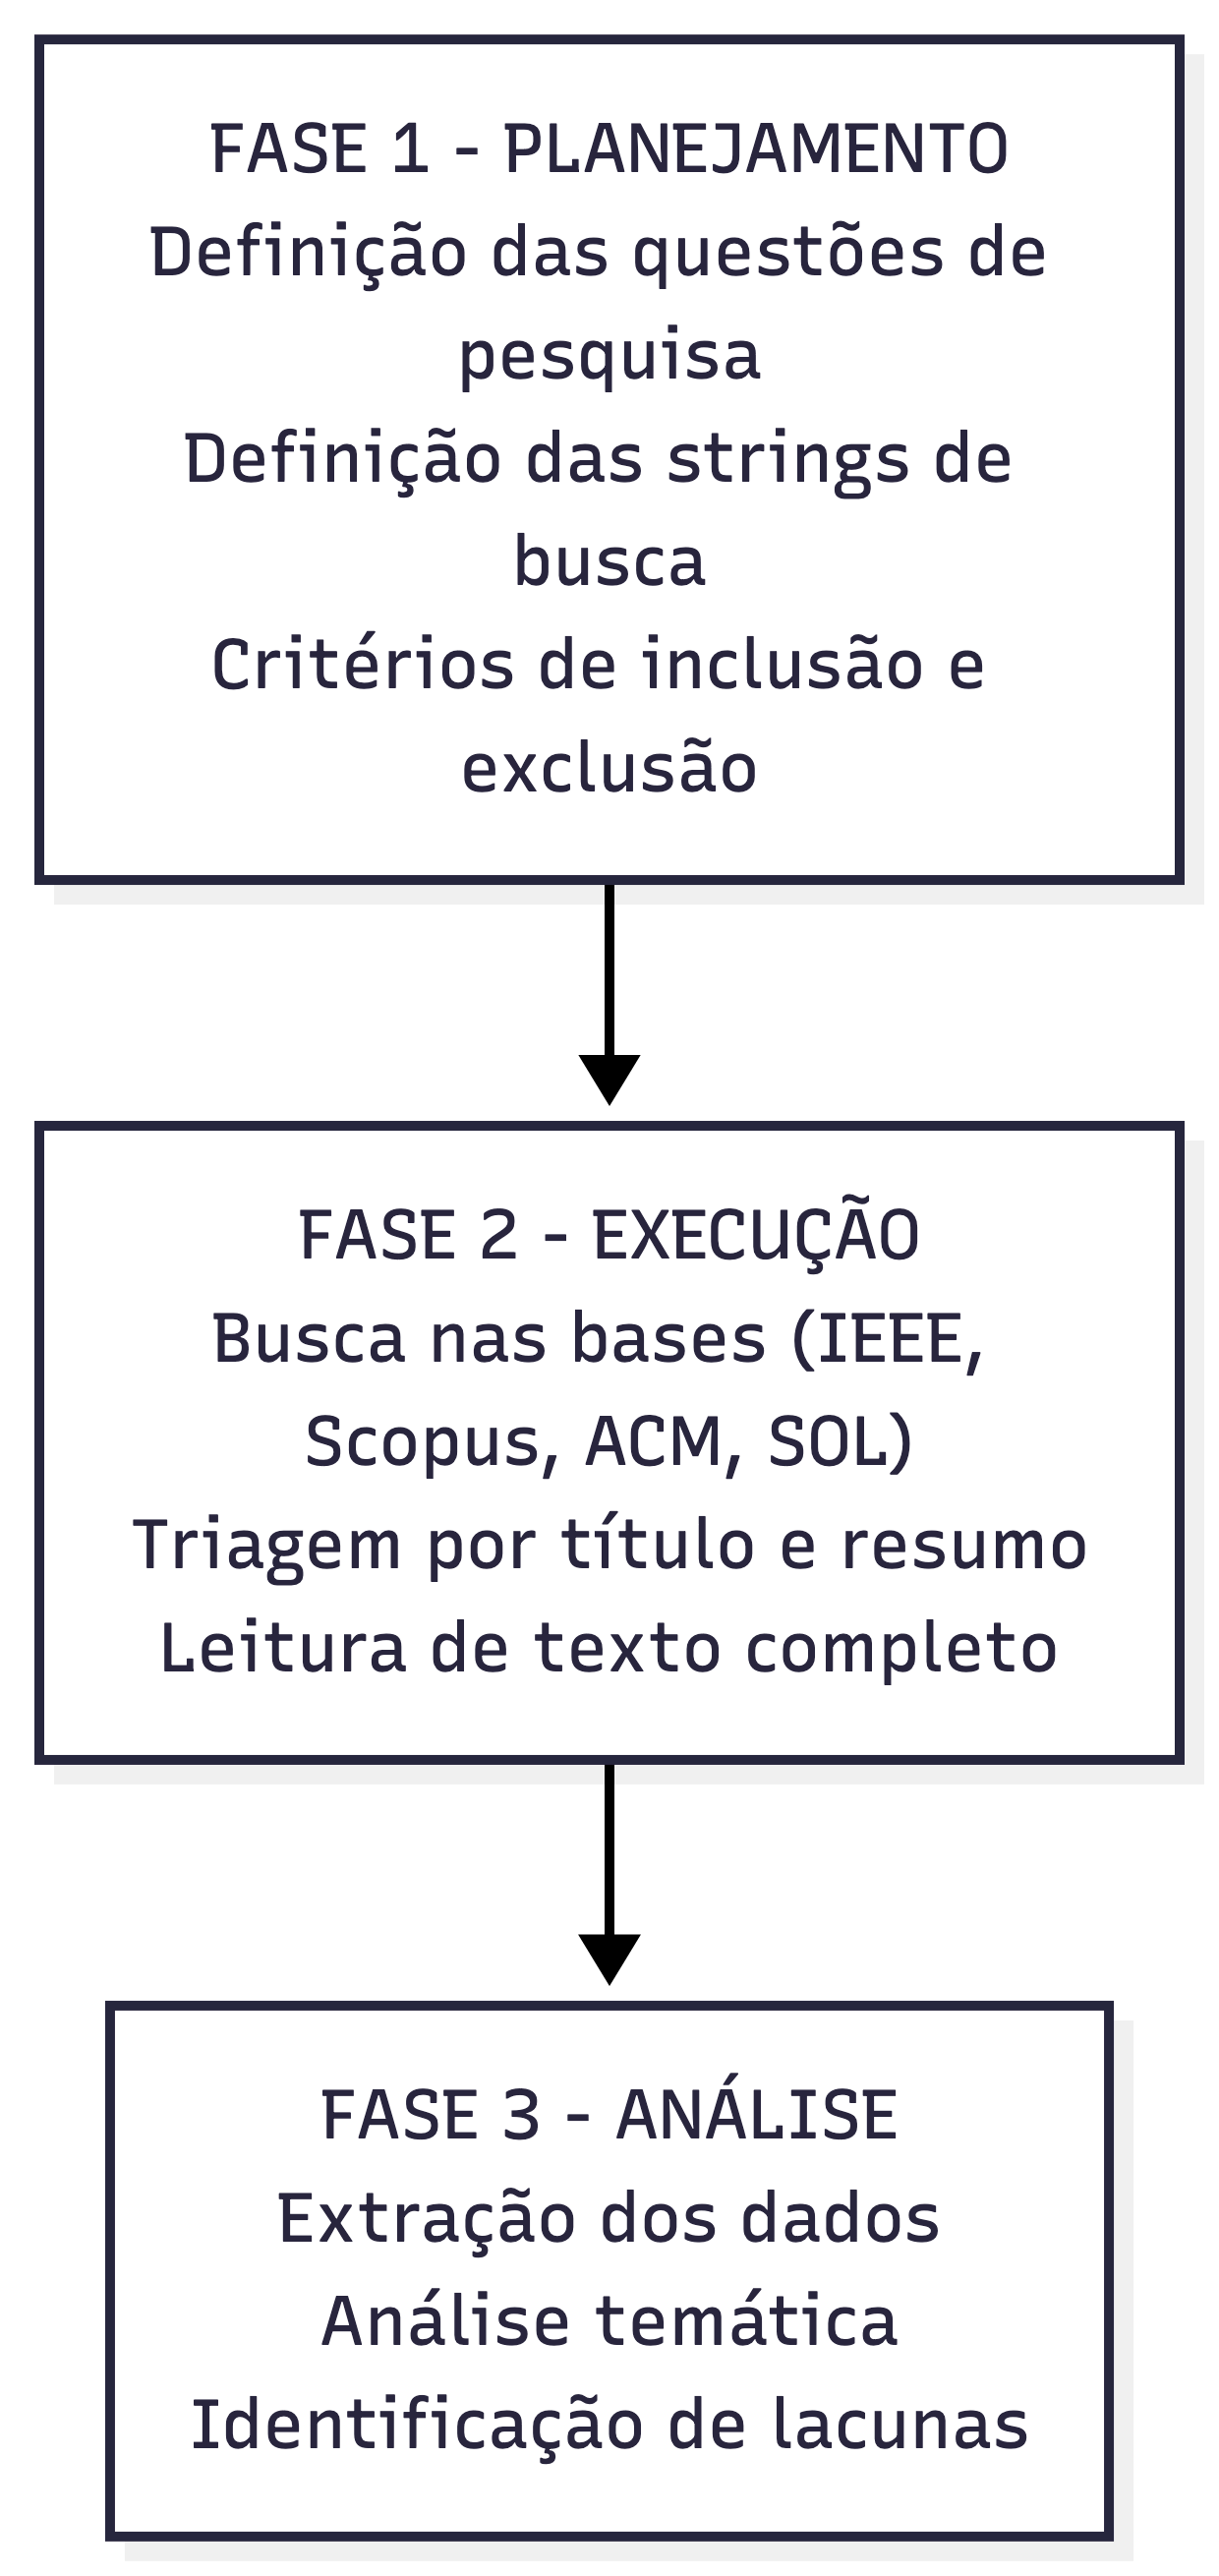
\includegraphics[width=0.5\textwidth]{imagens/fase_rsl.png}
    \fonte{Adaptado de Kitchenham (2004).}
\end{figure}

Para a organização e condução do mapeamento, utilizou-se a ferramenta \textit{Parsifal}\footnote{\url{https://parsif.al/}}, que oferece suporte computacional para a aplicação dos critérios de seleção e extração de dados.

\subsection{Planejamento}

Nesta etapa, definiu-se a necessidade do mapeamento e o protocolo de pesquisa \cite{Brereton2007}. O objetivo central foi responder às questões de pesquisa detalhadas no Quadro \ref{tab:questoes_pesquisa}, que orientaram a estratégia de busca.

\begin{quadro}[H]
    \centering
    \caption{Questões de Pesquisa do Mapeamento Sistemático}
    \label{tab:questoes_pesquisa}
    \begin{tabular}{p{3cm}p{10cm}}
    \toprule
    \textbf{ID da Questão} & \textbf{Questões de Pesquisa} \\
    \midrule
    Q1: & Quais técnicas de Inteligência Artificial ou PLN são mais utilizadas na literatura para a análise de dados parlamentares abertos? \\
    Q2: & Existem trabalhos que aplicam IA Generativa (LLMs) ou interfaces conversacionais (\textit{chatbots}) para facilitar o acesso do cidadão a dados legislativos? \\
    Q3: & Quais são as principais lacunas e desafios apontados pela literatura na democratização do acesso à informação parlamentar? \\
    Q4: & Como a literatura trata interação humano-dados e acessibilidade de informação legislativa? \\
    \bottomrule
    \end{tabular}
    \fonte{Produção da autora.}
\end{quadro}

Para responder a essas questões, foram definidos os campos de extração apresentados no Quadro \ref{tab:campo_extracao}.

\begin{quadro}[H]
    \centering
    \caption{Campos de Extração de Dados}
    \label{tab:campo_extracao}
    \begin{tabular}{p{10cm}}
    \toprule
    \textbf{Campo de Extração} \\
    \midrule
    Ano de Publicação \\
    Técnica/Método de IA/PLN Utilizado \\
    Uso de IA Generativa ou \textit{Chatbot}? \\
    Contexto Legislativo (Nacional vs. Internacional) \\
    Enfoque em Acessibilidade ou Interação Humano-Dados \\
    Desafios/Lacunas Identificados \\
    \bottomrule
    \end{tabular}
    \fonte{Produção da autora.}
\end{quadro}

\textbf{Fontes de Busca:}

Para esta pesquisa, a busca foi conduzida em cinco bases de dados de alto impacto internacional e nacional:

\begin{itemize}
    \item \textbf{IEEE Xplore:} Base multidisciplinar de Engenharia e Computação
    \item \textbf{Scopus:} Indexador de citações com cobertura de múltiplas disciplinas
    \item \textbf{ACM Digital Library:} Publicações especializadas em Ciência da Computação
    \item \textbf{Web of Science (WoS):} Base multidisciplinar de alto fator de impacto, incluída para ampliar a cobertura de publicações internacionais em Ciências da Computação e Sistemas de Informação
    \item \textbf{SOL - Biblioteca Digital da SBC:} Repositório da Sociedade Brasileira de Computação (\url{https://sol.sbc.org.br/}) para capturar produção científica nacional relevante
\end{itemize}

O escopo temporal compreendeu o período de 2014 a 2026, refletindo a evolução das políticas de dados abertos no Brasil e a emergência recente de aplicações baseadas em IA Generativa.

Data da busca: Maio de 2026.

As palavras-chave e \textit{strings} de busca utilizadas estão detalhadas nos Quadros \ref{tab:palavras_chave} e \ref{tab:string_busca}.

\begin{quadro}[H]
    \centering
    \caption{Palavras-Chave da Busca}
    \label{tab:palavras_chave}
    \begin{tabular}{p{5cm}p{8cm}}
    \toprule
    \textbf{Palavras-Chave (PT)} & \textbf{Termos em Inglês} \\
    \midrule
    Dados Parlamentares & Parliamentary Data, Legislative Data, Plenary Sessions \\
    IA Generativa & Generative Artificial Intelligence, LLM, Large Language Models \\
    Análise de Discursos & Information Extraction, Text Analysis, Speech Mining \\
    Dados Abertos & Open Government Data, Open Data \\
    Interface Conversacional & Chatbot, Conversational AI, Dialog Systems \\
    Acessibilidade de Dados & Data Accessibility, Data Literacy \\
    Transparência Legislativa & Legislative Transparency, Open Parliament \\
    \bottomrule
    \end{tabular}
    \fonte{Produção da autora.}
\end{quadro}

\begin{quadro}[H]
    \centering
    \caption{Strings de Busca (Conceituais)}
    \label{tab:string_busca}
    \begin{tabular}{p{13cm}}
    \toprule
    \textbf{String de Busca} \\
    \midrule
    (``Parliamentary Data" OR ``Legislative Data") AND (``Generative AI" OR ``Large Language Models" OR ``LLM" OR ``Chatbot") \\
    (``Open Government Data") AND (``Natural Language Processing" OR ``NLP" OR ``Text Mining") AND (``Parliament" OR ``Legislature") \\
    (``Legislative Transparency") AND (``Artificial Intelligence" OR ``Machine Learning") \\
    (``Data Accessibility") AND (``Chatbot" OR ``Conversational AI") \\
    \bottomrule
    \end{tabular}
    \fonte{Produção da autora.}
\end{quadro}

O Quadro \ref{tab:criterios} apresenta os critérios estabelecidos para filtrar os trabalhos.

\begin{quadro}[H]
    \centering
    \caption{Critérios de Inclusão e Exclusão}
    \label{tab:criterios}
    \begin{tabular}{p{6.5cm}p{6.5cm}}
    \toprule
    \textbf{Critérios de Inclusão} & \textbf{Critérios de Exclusão} \\
    \midrule
    CI1: Aborda IA/PLN/LLM para dados governamentais ou parlamentares. & CE1: Estudos duplicados em múltiplas bases. \\
    CI2: Discute transparência ou participação política em contexto legislativo. & CE2: Literatura cinzenta ou não revisada por pares. \\
    CI3: Aborda dados abertos em contexto público/legislativo. & CE3: Estudos secundários (revisões de revisões). \\
    CI4: Investiga interação humano-dados ou acessibilidade. & CE4: Artigos que abordam exclusivamente aspectos legais/políticos sem componente técnico. \\
    \bottomrule
    \end{tabular}
    \fonte{Produção da autora.}
\end{quadro}

\subsection{Execução e Resultados}

A execução seguiu o protocolo estabelecido, compreendendo identificação, seleção, elegibilidade e inclusão. A busca inicial nas cinco bases retornou 47 estudos: IEEE Xplore (0), Scopus (6), ACM Digital Library (39), Web of Science (2) e SOL/SBC (0). A ausência de retorno na SOL/SBC e no IEEE para as \textit{strings} aplicadas foi registrada como resultado negativo esperado — dado o recorte temporal e temático definido — e não implica ausência de produção nacional na área. Após remoção de 2 duplicatas e aplicação dos critérios de inclusão/exclusão (triagem por título e resumo, seguida de leitura de texto completo), selecionaram-se 7 trabalhos primários como mais relevantes para contextualizar esta dissertação.

O fluxo de seleção é detalhado na Figura \ref{fig:fluxograma_execucao}.

\begin{figure}[H]
    \centering
    \caption{Fluxograma de seleção dos estudos (PRISMA-ScR)}
    \label{fig:fluxograma_execucao}
    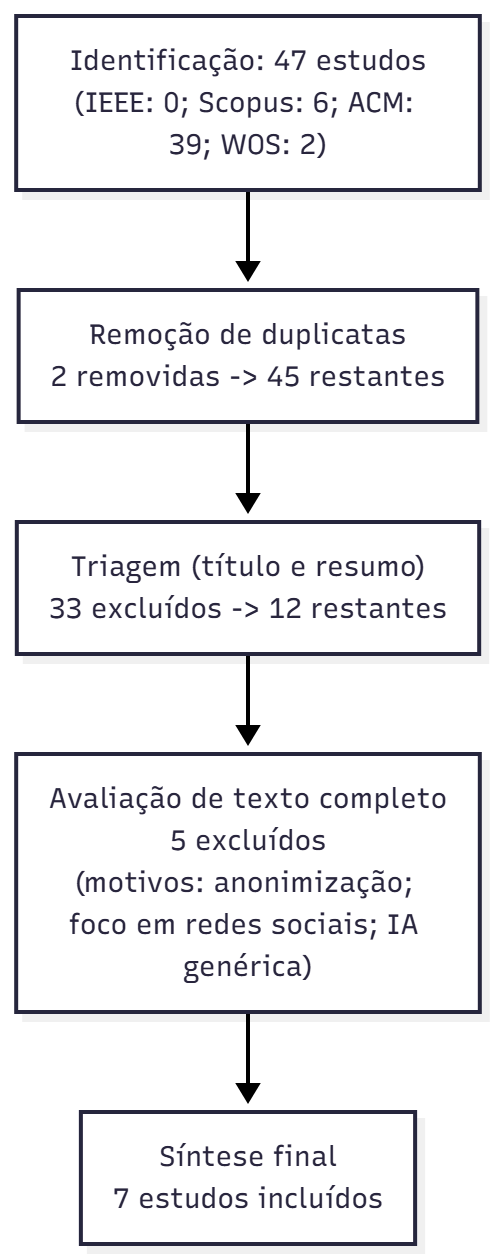
\includegraphics[width=0.5\textwidth]{imagens/fluxograma_execucao.png}
    \fonte{Produção da autora.}
\end{figure}

\section{Análise Temática dos Resultados}

Diferentemente de uma mera listagem de resumos, a análise temática busca identificar padrões, convergências e divergências entre os trabalhos, conectando-os explicitamente aos objetivos desta pesquisa e às lacunas identificadas.

\subsection{Tema 1: IA Generativa para Estruturação de Dados Legislativos}

Os trabalhos de Colombo et al. (2025), Colombo (2024) e Von Lucke e Frank (2025) convergem em um ponto fundamental: \textbf{modelos de linguagem generativa conseguem, quando bem orientados, transformar dados legislativos complexos em estruturas de conhecimento compreensíveis}.

\textbf{Especificidades de cada trabalho:}

\begin{itemize}
    \item \citeonline{Colombo2025} propõem um \textit{pipeline} assistido por LLM para construção automática de \textit{knowledge graphs} da legislação italiana. O trabalho demonstra que IA pode extrair entidades jurídicas (leis, artigos, interpretações) de textos legislativos não estruturados e organizá-las em grafos semânticos. Limitação: foca em estruturação técnica, não em acessibilidade para cidadãos.

    \item \citeonline{Colombo2024} aprofunda a discussão anterior, explorando explicitamente a sinergia entre grafos de conhecimento e LLMs para \textit{monitoring} de sistemas legislativos — rastreamento de como leis evoluem. Contribuição: metodologia de versionamento de legislação.

    \item \citeonline{VonLuckeFrank2025} analisam a aplicação prática de ferramentas como ChatGPT em parlamentos, levantando questões críticas sobre potencialidades (rapidez, síntese) e riscos (alucinação, imprecisão factual). Este trabalho é particularmente relevante pois trata de LLMs em contexto parlamentar e aponta desafios de confiabilidade.
\end{itemize}

\textbf{Padrão Emergente:} LLMs conseguem estruturar legislação, mas confiabilidade das respostas é crítica. A literatura aponta a necessidade de validação humana.

\textbf{Conexão com Este Trabalho:} Esta pesquisa avança ao (1) avaliar tecnicamente a confiabilidade das respostas geradas, (2) combinar estruturação de dados com interfaces visual e conversacional, (3) focar em dados parlamentares brasileiros.

\subsection{Tema 2: Interfaces Conversacionais para Acessibilidade}

\citeonline{Kim2025} descrevem o ``LegisFlow", uma interface conversacional com ``consciência temporal" para pesquisa jurídica na Coreia. Este trabalho é diretamente alinhado aos objetivos desta dissertação.

\textbf{Especificidades:}

\begin{itemize}
    \item Implementa chatbot para consultas em linguagem natural sobre legislação
    \item Incorpora noção de tempo (como leis mudaram ao longo do tempo)
    \item Avalia usabilidade com usuários reais
    \item Contexto: público coreano sem expertise jurídica
\end{itemize}

\textbf{Padrão Emergente:} Interfaces conversacionais reduzem barreira de entrada para acesso legislativo. Dimensão temporal é importante.

\textbf{Conexão e Diferenciação:} Este trabalho dialoga com o LegisFlow, mas dele se distingue deliberadamente. A interface conversacional, em si, não é a contribuição reivindicada --- ela já é demonstrada por Kim et al., inclusive com avaliação junto a usuários reais. O diferencial desta dissertação assenta-se em três eixos: (i) o contexto brasileiro e a língua portuguesa, ausentes naquele trabalho; (ii) a combinação de \textit{dashboard} visual e agente conversacional em um mesmo artefato, atendendo a padrões de uso distintos; e (iii) o foco explícito na rastreabilidade técnica das respostas, com instrumentação e métricas próprias, em vez da usabilidade percebida. Reconhece-se, em contrapartida, que este trabalho não avalia o impacto junto a usuários reais --- dimensão em que o LegisFlow avança e que aqui se delimita como trabalho futuro.

\subsection{Tema 3: Análise de Dados Legislativos com PLN Clássico}

\citeonline{Mendes2025} utilizam \textit{Topic Modeling} (técnica clássica de PLN, não IA Generativa) para analisar Pedidos de Acesso à Informação brasileiros. \citeonline{Bojars2019} apresentam ``LinkedSaeima", um dataset de dados abertos conectados (\textit{Linked Data}) do parlamento da Letônia.

\textbf{Padrão Emergente:} Abordagens clássicas de PLN conseguem extrair insights, mas requerem expertise técnica. IA Generativa oferece potencial para democratizar acesso.

\textbf{Conexão com Este Trabalho:} Enquanto esses trabalhos usam técnicas sofisticadas (Topic Modeling, RDF/Linked Data), o foco desta pesquisa é em acessibilidade para cidadãos não-especialistas. Essa é a lacuna que esta dissertação endereça.

\subsection{Tema 4: Desafios e Lacunas na Literatura}

\citeonline{PapadopoulosCharalabidis2020} aplicam PLN para extrair \textit{insights} de documentos de estratégias nacionais de IA, focando em mineração de textos governamentais. O trabalho, embora não focado em legislação, aponta desafios gerais na análise de textos públicos.

\textbf{Lacunas Identificadas Pela Literatura:}

\begin{enumerate}
    \item \textbf{Falta de foco em acessibilidade para cidadãos:} A maioria dos trabalhos trata estruturação técnica ou análise especializada, não democratização de acesso.

    \item \textbf{Confiabilidade de LLMs não é plenamente abordada:} Von Lucke e Frank apontam riscos, mas nenhum trabalho apresenta estratégia sistemática de validação.

    \item \textbf{Contexto brasileiro pouco explorado:} Dos 7 trabalhos, apenas Mendes et al. e Bojārs et al. abordam contexto nacional (coreano, letão, brasileiro). Falta pesquisa em português sobre legislação brasileira com IA Generativa.

    \item \textbf{Avaliação de respostas e rastreabilidade ainda é pouco explorada:} A literatura aponta riscos de alucinação e imprecisão factual em LLMs, mas ainda há espaço para protocolos de avaliação voltados à coerência entre respostas geradas e dados legislativos de origem.

    \item \textbf{Combinação Dashboard + Chatbot não é explorada:} Trabalhos tratam uma ou outra modalidade, raramente ambas integradas.
\end{enumerate}

\section{Lacunas Identificadas e Contribuições Desta Pesquisa}

Com base na análise sistemática, identificam-se as seguintes lacunas que esta pesquisa propõe-se a preencher:

\begin{enumerate}
    \item \textbf{Lacuna 1: Falta de foco em acessibilidade para cidadãos não-especialistas}
    \begin{itemize}
        \item \textbf{O que a literatura oferece:} Técnicas sofisticadas de IA para estruturação de legislação
        \item \textbf{O que está faltando:} Investigação de como essas técnicas podem ser comunicadas de forma compreensível ao cidadão médio
        \item \textbf{Como esta pesquisa aborda:} Design deliberado de interfaces acessíveis (Dashboard + Chatbot) e avaliação técnica de sua capacidade de organizar e consultar dados parlamentares
    \end{itemize}

    \item \textbf{Lacuna 2: Confiabilidade e validação de respostas IA não é sistemática}
    \begin{itemize}
        \item \textbf{O que a literatura oferece:} Identificação de riscos (alucinação, imprecisão)
        \item \textbf{O que está faltando:} Metodologia sistemática de validação antes de deploy em contexto cívico
        \item \textbf{Como esta pesquisa aborda:} Avaliação técnica rigorosa por meio de comparação com gabarito de referência, análise factual das respostas e verificação de rastreabilidade
    \end{itemize}

    \item \textbf{Lacuna 3: Contexto e idioma brasileiros pouco explorados}
    \begin{itemize}
        \item \textbf{O que a literatura oferece:} Exemplos internacionais (Itália, Coreia, Letônia)
        \item \textbf{O que está faltando:} Pesquisa em português sobre Senado Federal brasileiro
        \item \textbf{Como esta pesquisa aborda:} Dados reais da API do Senado Federal, legislação e dados parlamentares em língua portuguesa, contexto brasileiro até então ausente na literatura
    \end{itemize}

    \item \textbf{Lacuna 4: Avaliação factual e rastreável de respostas em linguagem natural}
    \begin{itemize}
        \item \textbf{O que a literatura oferece:} Discussões sobre potencial de LLMs e riscos de imprecisão
        \item \textbf{O que está faltando:} Protocolos explícitos para verificar se respostas geradas estão ancoradas em dados legislativos oficiais
        \item \textbf{Como esta pesquisa aborda:} Avaliação das respostas do AgentAI por cenários de consulta, comparação com dados oficiais e análise de rastreabilidade
    \end{itemize}

    \item \textbf{Lacuna 5: Integração de múltiplas modalidades de interação}
    \begin{itemize}
        \item \textbf{O que a literatura oferece:} Dashboards OU Chatbots, raramente ambos
        \item \textbf{O que está faltando:} Investigação de como diferentes modalidades se complementam para diferentes usuários
        \item \textbf{Como esta pesquisa aborda:} Design deliberado de Dashboard + Chatbot com avaliação de como ambos contribuem ao acesso democrático
    \end{itemize}
\end{enumerate}

\section{Conclusões do Mapeamento Sistemático}

O mapeamento revela um campo em formação: trabalhos sobre IA Generativa aplicada a legislação são recentes (predominantemente pós-2022), concentrados em contextos europeus e asiáticos, e orientados predominantemente à estruturação técnica — não à acessibilidade para cidadãos comuns. A ausência de trabalhos em português sobre dados parlamentares brasileiros com LLMs, combinada à falta de protocolos sistemáticos para avaliação de rastreabilidade e qualidade factual de respostas geradas, configura o espaço em que esta dissertação se insere.

É importante registrar uma limitação do próprio mapeamento: o corpus de 7 estudos primários selecionados é pequeno para afirmações categóricas sobre o estado da área, e a forte concentração de retornos em uma única base (ACM Digital Library) pode enviesar as lacunas identificadas, que devem, portanto, ser lidas como indícios e não como conclusões definitivas. Essa limitação pode refletir tanto a emergência da temática quanto restrições das \textit{strings} de busca utilizadas. A reexecução conduzida na RSL desta dissertação ampliou o escopo de bases consultadas e documentou, em apêndice, as \textit{strings} exatas aplicadas em cada base, com os respectivos números de retorno e filtros --- requisitos para a plena reprodutibilidade, conforme as diretrizes de Kitchenham \cite{Kitchenham2004}. A complementação por \textit{snowballing} --- para frente e para trás --- a partir dos estudos incluídos não foi conduzida nesta versão e fica registrada como trabalho futuro.


\chapter{Desenvolvimento e Resultados Preliminares} % Sugestão de ajuste no título
\label{cap:desenvolvimento}
Neste capítulo, detalha-se o estágio atual do projeto e o planejamento para a conclusão da dissertação. Como esta proposta é apresentada em um estágio avançado do mestrado, a fase de construção do artefato (aplicação \textit{web}, \textit{backend} e integração com IA) já se encontra concluída (Fase de Design e Desenvolvimento), permitindo que os esforços futuros se concentrem na validação científica (Fase de Avaliação) e na escrita final.

\section{Estágio Atual do Desenvolvimento}

Sob a ótica da \textit{Design Science Research}, o artefato computacional proposto já atingiu um nível de maturidade funcional que permite a execução de testes. As seguintes etapas do ciclo de pesquisa foram concluídas:

\begin{itemize}
    \item \textbf{Identificação do Problema e Motivação:} Mapeamento das dificuldades de acesso aos dados brutos do Senado Federal e definição da relevância para o controle social e participação democrática.

    \item \textbf{Definição da Solução:} Projeto de uma arquitetura baseada em Dashboard (visualização) + Chatbot (interação conversacional) para reduzir barreiras cognitivas ao acesso legislativo.

    \item \textbf{Design e Desenvolvimento:} Implementação completa dos módulos de coleta (ETL via API Senado), análise (Mistral 7B Instruct em ambiente local) e interface (\textit{Streamlit} com \textit{Plotly}), resultando em um protótipo funcional capaz de processar dados reais.

    \item \textbf{Demonstração:} Validação técnica preliminar mostrando que o artefato consegue processar dados parlamentares e gerar respostas coerentes.
\end{itemize}

A aplicação encontra-se implantada em ambiente de homologação, processando dados da API do Senado Federal e respondendo a consultas em linguagem natural. Esse estágio habilita a fase de avaliação técnica do artefato, com foco em qualidade dos dados processados, acurácia da classificação temática, qualidade factual das respostas e rastreabilidade das informações geradas.

\section{Arquitetura e Componentes do Artefato}

\subsection{Camada de Dados: Coleta e Processamento}

A coleta de dados é efetuada via API de Dados Abertos do Senado Federal \cite{SenadoFederal_s_d}. O processo de ETL (\textit{Extract, Transform, Load}) é automatizado e inclui:

\begin{itemize}
    \item \textbf{Extração:} Utilização da biblioteca \textit{Requests} \cite{RequestsLib} para requisição de dados brutos (XML/JSON) dos \textit{endpoints} da API Swagger, mapeando informações sobre sessões legislativas, discursos, votações e senadores.

    \item \textbf{Transformação:} Conversão e limpeza dos dados utilizando \textit{Pandas} \cite{PandasLib}, normalizando formatos, removendo duplicatas, preenchendo valores ausentes e estruturando informações em tabelas relacionais otimizadas para análise.

    \item \textbf{Carregamento:} Os dados transformados são mantidos em memória durante a execução e persistidos em um \textit{cache} em arquivo (\texttt{outputs/materias\_cache.json}), que funciona como \textit{snapshot} local: requisições repetidas à API são evitadas quando o mesmo período legislativo já foi coletado, e esse \textit{snapshot} pode ser versionado para assegurar a reprodutibilidade da avaliação sobre um corpus congelado.
\end{itemize}

A atualização do corpus ocorre sob demanda, mediante reexecução do \textit{pipeline} para o período desejado; neste estágio de prototipação não há um agendamento automático em produção. Para fins de avaliação científica, adota-se deliberadamente um \textit{snapshot} congelado e versionado dos dados, de modo que os experimentos sejam reproduzíveis sobre exatamente o mesmo conjunto --- condição necessária para que o gabarito de referência permaneça estável entre execuções.

\subsection{Camada de Inteligência: Análise com Mistral 7B}

O núcleo analítico utiliza o modelo Mistral 7B Instruct \cite{MistralAI2024}, executado em ambiente local. A justificativa dessa escolha --- privacidade e soberania de dados, replicabilidade, custo e adequação de desempenho ---, bem como a comparação com modelos proprietários e com outros modelos abertos, foi apresentada na fundamentação teórica (Seção~\ref{subsec:escolha_modelo}) e não é aqui repetida.

Do ponto de vista de implementação, o modelo é servido localmente por um \textit{runtime} de inferência que expõe uma API compatível com o padrão OpenAI em \texttt{localhost} (na configuração de referência, o LM Studio em \texttt{http://localhost:1234/v1}). O artefato comunica-se com o modelo exclusivamente por essa interface local: nenhum dado legislativo é transmitido a servidores externos, de modo que a soberania de dados é preservada mesmo havendo uma camada de \textit{serving} compatível com OpenAI. Essa padronização da interface é também o que torna o componente de linguagem modular e substituível por outro modelo sem alteração dos demais estágios.

O modelo é utilizado para duas funções críticas:

\begin{itemize}
    \item \textbf{Classificação Temática:} Engenharia de \textit{prompts} estruturados instrui o modelo a categorizar discursos legislativos em temas predefinidos (Saúde, Educação, Infraestrutura, Segurança, etc.). A classificação permite organização e análise dos debates por assunto.

    \item \textbf{Motor de Resposta (Recuperação Estruturada com Geração Aumentada):} O módulo recebe perguntas do usuário em linguagem natural via Chatbot, recupera da base em memória um subconjunto de registros relevantes à pergunta (busca estruturada por palavras-chave sobre os dados mantidos em cache de sessão) e instrui o Mistral 7B a gerar respostas contextualizadas e didáticas, fundamentadas nesses registros e citando-os por identificador estável (por exemplo, \texttt{[D1]} para discursos e \texttt{[V1]} para votações).
\end{itemize}

\subsection{Camada de Apresentação: Interfaces Acessíveis}

Para materializar o acesso democrático aos dados, desenvolveu-se uma interface \textit{web} utilizando o \textit{framework Streamlit} \cite{Streamlit2024}, oferecendo dois modos de interação complementares:

\subsubsection{Dashboard Visual}

Gráficos interativos gerados com \textit{Plotly} \cite{Plotly2024} permitem exploração visual de tendências legislativas. O design segue o mantra de Shneiderman \cite{Shneiderman1996}: "primeiro o panorama geral, depois zoom e filtros, e então detalhes sob demanda".

\textbf{Exemplos de visualizações disponíveis:}

\begin{itemize}
    \item Tendências de votação ao longo do tempo (linha temporal)
    \item Distribuição de votos por tema (gráfico de barras)
    \item Padrões de voto de senadores específicos (matriz ou radar)
    \item Comparação entre posições de diferentes grupos parlamentares (gráficos comparativos)
\end{itemize}

O Dashboard permite que usuários explorem livremente, filtrem por tema, senador ou período, e identifiquem padrões visuais em dados legislativos.

O uso do Streamlit é uma escolha compatível com o estágio de prototipação científica do artefato, pois permite rápida construção de interfaces interativas para análise de dados. Entretanto, reconhece-se que o framework possui limitações para uso em produção em larga escala, especialmente em autenticação, controle fino de permissões, escalabilidade e separação entre camadas de serviço. Assim, neste trabalho, o Streamlit é tratado como tecnologia de prototipação e demonstração do artefato, não como decisão definitiva para implantação institucional.

\subsubsection{Chatbot Conversacional}

Interface de \textit{chat} que abstrai a complexidade dos dados legislativos, permitindo consultas em linguagem natural:

\textbf{Exemplos de perguntas que o usuário pode fazer:}

\begin{itemize}
    \item "Como votou o Senador [Nome] sobre educação?"
    \item "Qual foi o resultado da votação em [Projeto de Lei]?"
    \item "Quais são os temas mais debatidos em 2025?"
    \item "Como o partido [X] votou no projeto sobre saúde?"
    \item "Qual senador votou diferente de seu partido nesta votação?"
\end{itemize}

O Chatbot traduz perguntas em linguagem comum para operações sobre a base de dados em memória, recupera as informações relevantes e retorna respostas em linguagem natural acessível a cidadãos sem expertise legislativa ou tecnológica. A Figura \ref{fig:tela_chatbot} ilustra a interface conversacional em operação com dados reais do Senado Federal.

\begin{figure}[H]
    \centering
    \caption{Interface do Agente Conversacional (Chatbot) do AgentAI}
    \label{fig:tela_chatbot}
    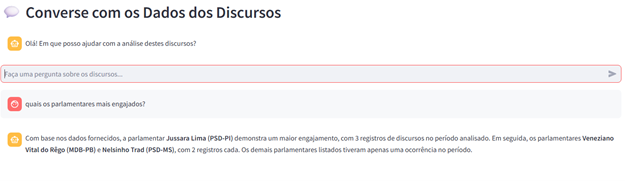
\includegraphics[width=0.9\textwidth]{imagens/tela_chatbot.png}
    \fonte{Produção da autora.}
\end{figure}

\subsection{Rastreabilidade das Respostas}

Para que o agente conversacional não opere como uma "caixa-preta", o artefato foi instrumentado de modo a tornar explícita a ligação entre cada resposta e os dados que a fundamentaram. Esse mecanismo, já implementado no protótipo, opera em dois níveis complementares:

\begin{itemize}
    \item \textbf{No artefato (rastreabilidade para o usuário):} a etapa de \textit{retrieval} seleciona, para cada pergunta, um subconjunto de registros da base e atribui a eles identificadores curtos e estáveis (\texttt{[D1]}, \texttt{[D2]}, \ldots\ para discursos; \texttt{[V1]}, \texttt{[V2]}, \ldots\ para votações). O \textit{prompt} instrui o modelo a fundamentar a resposta exclusivamente nesses registros e a citá-los por identificador, sendo vedado referenciar identificadores fora da lista recuperada. A interface exibe, junto a cada resposta, um painel "Fontes utilizadas" com a tabela dos registros efetivamente recuperados, preservando também o código oficial do Senado de cada item. O mecanismo aplica-se tanto ao \textit{chat} de discursos quanto ao de votações.

    \item \textbf{Para avaliação (instrumentação de medição):} cada consulta gera um registro estruturado em \textit{log} (arquivo \texttt{qa\_trace.jsonl}) contendo a pergunta, os identificadores das fontes recuperadas, os códigos oficiais correspondentes e a resposta gerada. Sobre esse \textit{log}, um módulo de avaliação calcula indicadores de rastreabilidade, também acessíveis por um painel dedicado na própria interface. Esse encadeamento --- recuperação, citação, registro e medição --- funciona de ponta a ponta; a medição sobre o conjunto de cenários definido, incluindo a verificação de suporte semântico das citações, integra a fase de avaliação ainda em execução, detalhada no Capítulo~\ref{cap:metodologia}.
\end{itemize}

\section{Fluxo de Funcionamento do Sistema}

O sistema opera conforme descrito abaixo:

\begin{enumerate}
    \item \textbf{Inicialização:} Aplicação \textit{Streamlit} carrega dados pré-processados da API do Senado Federal, mantendo-os em memória com cache de sessão.

    \item \textbf{Interação Usuário - Dashboard:} Usuário pode explorar Dashboard sem necessidade de entrada, aplicando filtros interativos para ver visualizações customizadas.

    \item \textbf{Interação Usuário - Chatbot:} Usuário digita pergunta em linguagem natural.

    \item \textbf{Processamento:}
    \begin{itemize}
        \item Sistema faz \textit{retrieval} de dados relevantes (busca estruturada por palavras-chave sobre a base local)
        \item Constrói contexto com os dados recuperados
        \item Instrui Mistral 7B com \textit{prompt} que inclui: pergunta do usuário, contexto de dados e instruções para responder de forma didática
    \end{itemize}

    \item \textbf{Resposta:} Mistral 7B gera resposta em linguagem natural, citando por identificador (\texttt{[D1]}, \texttt{[V1]}, etc.) quais registros recuperados foram utilizados.

    \item \textbf{Exibição:} A resposta é exibida no Chatbot, acompanhada do painel "Fontes utilizadas" que lista os registros recuperados. O usuário pode fazer pergunta de acompanhamento.
\end{enumerate}

\section{Dados Legislativos Utilizados}

O artefato processa dados da API de Dados Abertos do Senado Federal, incluindo:

\begin{itemize}
    \item \textbf{Senadores:} Nomes, partidos, estados, contatos
    \item \textbf{Sessões Plenárias:} Datas, tipo (ordinária, extraordinária, etc.)
    \item \textbf{Discursos:} Texto completo, senador autor, data, tema (quando disponível)
    \item \textbf{Votações:} Descrição da matéria votada, resultado, votos individuais de cada senador
\end{itemize}

Os dados cobrem o período de 2024 a 2026 e permitem a investigação de padrões legislativos contemporâneos. Esse recorte temporal poderá ser ampliado na etapa final da pesquisa, conforme a disponibilidade da API e os limites de processamento do ambiente local.

\section{Status de Conclusão das Fases DSR}

Conforme a metodologia Design Science Research (Cap.\ \ref{cap:metodologia}), o projeto encontra-se no seguinte estágio:

\begin{quadro}[H]
    \centering
    \caption{Progresso das Fases de Design Science Research}
    \label{quad:fases_dsr}
    \begin{tabular}{|p{4.5cm}|>{\centering\arraybackslash}p{2.8cm}|p{7cm}|}
        \hline
        \textbf{Fase DSR} & \textbf{Status} & \textbf{Descrição} \\
        \hline
        1. Identificação do Problema & Concluída & Problema definido, fundamentado em literatura \\
        \hline
        2. Objetivos da Solução & Concluída & Objetivos do artefato claramente especificados \\
        \hline
        3. Design e Desenvolvimento & Concluída & Artefato implementado e funcional \\
        \hline
        4. Demonstração & Concluída & Artefato operacional em ambiente de homologação \\
        \hline
        5. Avaliação & \textit{Em Execução} & Testes técnicos, factuais e de rastreabilidade planejados (Trim. 2-3) \\
        \hline
        6. Reflexão e Aprendizados & \textit{Planejada} & A executar após fase de avaliação (Trim. 3-4) \\
        \hline
    \end{tabular}
    \fonte{Produção da autora.}
\end{quadro}

\section{Cronograma de Execução da Dissertação}

O planejamento temporal das fases finais --- com foco na Avaliação rigorosa (Fase 5) e na produção textual até a defesa, prevista para janeiro de 2027 --- é apresentado de forma consolidada no Capítulo~\ref{cap:metodologia} (Quadro~\ref{quad:cronograma_metodologia}), evitando-se aqui a duplicação do cronograma. Esta seção registra apenas o encadeamento das próximas atividades imediatas, detalhado a seguir.

\section{Próximas Ações Imediatas (Próximas 8 Semanas)}

\begin{enumerate}
    \item Implementar melhorias apontadas pelo parecer de qualificação
    \item Finalizar dataset de controle para experimento de acurácia
    \item Preparar o conjunto de cenários representativos de consulta
    \item Executar primeira rodada de teste técnico (IA vs. Gabarito)
    \item Documentar detalhes finais do protocolo de avaliação técnica
\end{enumerate}


\chapter{Resultados da Avaliação}
\label{cap:resultados}
Este capítulo reporta os resultados da avaliação de geração do AgentAI, executada conforme o protocolo da Fase 5 detalhado no Capítulo~\ref{cap:metodologia} (Metodologia). A avaliação cobre as cláusulas (b) --- coerência factual das respostas --- e (c) --- rastreabilidade --- da hipótese de pesquisa. A cláusula (a), relativa à classificação temática comparada a uma linha de base por palavras-chave, ainda não foi avaliada: essa frente permanece planejada e sua execução integra o cronograma (Quadro~\ref{quad:cronograma_metodologia}), constituindo limitação assumida desta versão dos resultados e não um achado a omitir.

Adianta-se o argumento central, que não é a eleição de um modelo vencedor: as métricas automáticas \textit{saturam} nos quatro modelos avaliados --- integridade referencial $1{,}00$ e taxa de alucinação $0{,}00$ em todos ---, de modo que o \textbf{suporte semântico}, obtido por anotação humana, é o único eixo capaz de discriminar a qualidade das respostas. O caso da pergunta Q04 (Seção~\ref{sec:res_q04}) demonstra concretamente que uma resposta com métrica automática perfeita pode ter suporte semântico baixo. Como esse fenômeno se sustenta nos quatro modelos, o resultado é melhor lido como evidência da \textit{robustez do protocolo de avaliação} do que como ranqueamento de geradores.

\section{Configuração Experimental}

\subsection{Corpus de Avaliação}
A avaliação recaiu sobre um \textit{snapshot} congelado de 152 discursos do Senado Federal, coletados entre 5 e 16 de maio de 2025 (nove datas distintas). Cada registro contém o resumo do discurso e o tema atribuído (categoria fechada), sem o texto integral. Sobre esse corpus, definiu-se \textit{a priori} um conjunto de 40 perguntas estratificadas em cinco classes: 14 factuais diretas, 8 de agregação/contagem, 6 de comparação, 4 de busca por tema e 8 sem resposta no corpus. Estas últimas testam a robustez do gerador --- isto é, se ele reconhece a ausência de informação em vez de fabricá-la. O congelamento do corpus, da recuperação e dos hiperparâmetros assegura que qualquer diferença observada seja atribuível ao modelo gerador.

Cabe registrar que o motor de resposta emprega \textbf{recuperação estruturada com geração aumentada} por correspondência de palavra-chave, e não recuperação vetorial densa. As referências apresentadas nas respostas na forma \texttt{[D1]}, \texttt{[D2]} etc. são identificadores locais e posicionais por consulta --- isto é, apontam para a $k$-ésima fonte recuperada naquela pergunta ---, e não os identificadores de discurso originais do corpus; a conferência de suporte das citações foi feita contra a evidência \textit{gold} da pergunta.

\subsection{Modelos, Hardware e Quantização}
Foram avaliados quatro modelos de linguagem abertos, todos executados localmente no \textit{runtime} LM Studio: Mistral 7B Instruct v0.3 \cite{Jiang2023}, Qwen2.5 7B Instruct, Llama 3.1 8B Instruct e Gemma 2 9B Instruct. Mantém-se o Mistral 7B como o modelo do artefato por razões de replicabilidade, soberania de dados e sustentabilidade operacional já justificadas na fundamentação (Seção~\ref{subsec:escolha_modelo}); os demais entram aqui como termos de comparação sob condição idêntica.

Todos os quatro modelos foram executados na mesma quantização \textbf{Q4\_K\_M} (paridade confirmada pelos arquivos \texttt{.gguf}) e no mesmo equipamento: CPU AMD Ryzen 7 5700X (8 núcleos), 32~GB de RAM e GPU NVIDIA RTX 4060 Ti de 8~GB, sob Windows de 64 bits. A identidade de \textit{hardware} e de quantização entre as coletas é a condição que torna as métricas de latência e \textit{throughput} comparáveis entre os modelos; registre-se, contudo, que o consumo efetivo de VRAM e o regime de \textit{offload} de cada execução não foram instrumentados.

Um quinto modelo, o Sabiá-7B, foi \textbf{excluído} da comparação por incompatibilidade de janela de contexto: ele aceita no máximo 2048 \textit{tokens}, ao passo que os \textit{prompts} da tarefa (trechos recuperados, pergunta e instruções) ultrapassam 4000 \textit{tokens}. Incluí-lo exigiria truncar pela metade o contexto recuperado, violando o princípio de manter tudo fixo exceto o modelo e confundindo o efeito do gerador com o do \textit{handicap} de contexto. A janela de contexto é, portanto, um critério de elegibilidade anterior à avaliação de qualidade.

\subsection{Condição de Geração}
As gerações foram realizadas com temperatura $0{,}1$. Quanto à \textit{seed}, embora o \textit{script} de coleta envie o valor 42 no \textit{payload}, o LM Studio manteve o \textit{toggle} de \textit{seed} aleatória ativo nas quatro coletas, de modo que esse valor foi sobrescrito e a \textit{seed} \textbf{não foi efetivamente controlada} no \textit{runtime} de inferência. Não se afirma, portanto, determinismo por \textit{seed} fixa nem reprodutibilidade \textit{byte}-idêntica --- que o \textit{runtime} local não garante mesmo com \textit{seed} fixa, por não-determinismo de GPU. O que se assegura é a \textbf{uniformidade da condição}: os quatro modelos foram executados sob a mesma configuração (temperatura $0{,}1$ e \textit{seed} não controlada), o que preserva a validade da comparação. Por essa razão, métricas sensíveis à variação entre execuções --- sobretudo a recusa em perguntas sem resposta --- são reportadas em agregado sobre o conjunto de perguntas, nunca a partir de uma única pergunta.

\section{Resultados Quantitativos Agregados}

O Quadro~\ref{tab:comparativo_modelos} consolida as métricas por modelo ($n = 40$ perguntas por modelo, 160 anotações ao todo). As médias de suporte semântico, completude, português formal e a contagem de recusa correta provêm da anotação humana cega; integridade referencial, taxa de alucinação e \textit{throughput} provêm da instrumentação automática.

\begin{quadro}[H]
    \centering
    \caption{Avaliação comparativa dos quatro modelos geradores ($n = 40$ por modelo; quantização Q4\_K\_M)}
    \label{tab:comparativo_modelos}
    \resizebox{\textwidth}{!}{%
    \begin{tabular}{lccccccc}
        \toprule
        \textbf{Modelo} & \textbf{Suporte sem.} & \textbf{Recusa} & \textbf{PT formal} & \textbf{Completude} & \textbf{Tokens/s} & \textbf{Integ. ref.} & \textbf{Alucinação} \\
         & \textbf{(1--4)} & \textbf{(/8)} & \textbf{(1--5)} & \textbf{(1--5)} & \textbf{(mediana)} & & \\
        \midrule
        Mistral 7B Instruct v0.3 & 2,62 & 6/8 & 4,72 & 4,20 & 29,6 & 1,00 & 0,00 \\
        Qwen2.5 7B Instruct      & 2,90 & 5/8 & 4,85 & 4,12 & 23,1 & 1,00 & 0,00 \\
        Llama 3.1 8B Instruct    & 2,73 & 7/8 & 4,90 & 4,00 & 29,6 & 1,00 & 0,00 \\
        Gemma 2 9B Instruct      & 3,17 & 6/8 & 4,95 & 3,95 & 4,15 & 1,00 & 0,00 \\
        \bottomrule
    \end{tabular}%
    }
    \fonte{Produção da autora.}
\end{quadro}

\section{Saturação das Métricas Automáticas e o Suporte Semântico como Eixo Discriminante}

A integridade referencial e a taxa de alucinação atingiram o teto nos quatro modelos: todas as citações apontavam para fontes efetivamente recuperadas (integridade $1{,}00$) e nenhuma referenciava registro fora da janela recuperada (alucinação $0{,}00$). Esse resultado \textbf{valida o \textit{pipeline}} de recuperação e citação, mas, por saturar, não discrimina a qualidade das respostas: as duas métricas automáticas não distinguem os modelos entre si. A adequação ao português formal comporta-se de modo análogo, concentrada na faixa $4{,}72$--$4{,}95$, alta e pouco discriminante.

A discriminação recai, assim, sobre o suporte semântico anotado, no qual os modelos se ordenam como Gemma~2 ($3{,}17$), Qwen2.5 ($2{,}90$), Llama~3.1 ($2{,}73$) e Mistral ($2{,}62$). É preciso enfatizar que essas \textbf{diferenças são modestas}: todas se situam na faixa entre ``correta no núcleo, com lacunas'' e ``integralmente sustentada''. Como a anotação foi conduzida por avaliador único e sem cálculo de concordância interanotador (Kappa de Cohen), \textbf{não se afirma significância estatística nem dominância} de qualquer modelo; os valores caracterizam tendências, não um veredito. O ponto metodológico que se sustenta com robustez é outro: a distinção entre uma integridade referencial que satura e um suporte semântico que varia revela que a primeira mede a integridade da \textit{referência} (o identificador existe na janela?), enquanto o segundo mede a integridade do \textit{conteúdo} (a fonte sustenta o que foi dito?).

\section{O Caso Q04: Métrica Automática Perfeita com Suporte Semântico Baixo}
\label{sec:res_q04}

A pergunta Q04 --- ``Qual senador discursou sobre o aniversário de 35 anos da Conab?'' --- ilustra de forma concreta a insuficiência das métricas automáticas. Na resposta do Mistral, todas as referências citadas estavam dentro da janela recuperada, resultando em integridade referencial $1{,}00$ e alucinação $0{,}00$. A resposta, porém, continha erro semântico relevante: associava contagens fabricadas (``duas sessões''; outro parlamentar com ``três discursos sobre a Conab'') e grafava incorretamente o nome do parlamentar. Na anotação cega, recebeu \textbf{suporte semântico~2} --- erro relevante --- apesar da pontuação automática perfeita.

O contraste na mesma pergunta torna o argumento robusto entre modelos: o Qwen2.5 identificou corretamente o parlamentar e obteve \textbf{suporte~4}, enquanto Llama~3.1 e Gemma~2 ficaram em suporte~3 (corretos no núcleo, mas com imprecisões ou resposta genérica). Ou seja, sob métricas automáticas idênticas ($1{,}00$ / $0{,}00$ para os quatro), o suporte semântico separou uma resposta incorreta de uma correta. O caso demonstra empiricamente por que a anotação humana é indispensável e por que a avaliação de qualidade não pode se apoiar apenas na integridade referencial.

\section{Recusa Correta nas Perguntas sem Resposta no Corpus}

Nas 8 perguntas sem resposta no corpus, a recusa correta --- o reconhecimento explícito da ausência de dados --- foi de 7/8 para o Llama~3.1, 6/8 para Mistral e Gemma~2 e 5/8 para o Qwen2.5. Esses valores só emergem da leitura humana: o proxy automático de recusa (heurística ``ausência de citação $=$ recusa'') subestima sistematicamente a robustez, pois os modelos costumam reconhecer a ausência em prosa (``não foi registrado nos discursos analisados'') e, ainda assim, citar uma fonte de contexto, o que faz o proxy contabilizar indevidamente uma não-recusa. No caso do Mistral, por exemplo, o proxy automático marcou apenas 1/8, contra os 6/8 confirmados pela anotação humana. Reporta-se, portanto, a recusa automática como um piso, e a robustez real como aquela aferida por leitura humana.

\section{Discussão}

\subsection{Robustez do Achado entre Modelos}
O fato de os quatro modelos saturarem as métricas automáticas e de o fenômeno do caso Q04 se reproduzir independentemente do gerador confere robustez ao achado central: a avaliação de respostas ancoradas em dados não pode se apoiar em métricas de integridade de referência, que tendem a saturar, sendo necessária a verificação de suporte semântico do conteúdo. Esse resultado é uma propriedade do protocolo de avaliação, sustentada em quatro arquiteturas distintas, e não uma característica de um modelo isolado.

\subsection{Custo de Inferência e o \textit{Trade-off} Qualidade--Custo}
A leitura conjunta de qualidade e custo de inferência revela uma tensão. O Gemma~2, que lidera o suporte semântico, foi também o mais lento na geração por ampla margem: $4{,}15$ \textit{tokens}/s observados, contra $23$--$30$ \textit{tokens}/s dos modelos 7--8B, sob o mesmo \textit{hardware} e a mesma quantização Q4\_K\_M. Reporta-se essa diferença de forma descritiva: como o consumo de VRAM e o regime de \textit{offload} não foram instrumentados, não se isola aqui a causa do custo mais alto --- que pode refletir o maior porte do modelo, características de sua arquitetura ou o comportamento do \textit{runtime} local. A escolha de modelo configura-se, ainda assim, como um \textit{trade-off} entre qualidade e custo, e não como dominância simples: o ganho modesto de suporte semântico do Gemma vem acompanhado de um custo de geração várias vezes maior. As implicações dessa tensão para a eventual seleção de outro gerador --- viabilizada pela arquitetura modular do artefato --- são discutidas entre os trabalhos futuros, no capítulo de considerações, permanecendo o Mistral 7B como o modelo do artefato por replicabilidade.

\subsection{Limitações}
Reconhecem-se as seguintes limitações desta avaliação. Primeiro, a anotação foi conduzida por \textbf{anotador único}, em condição cega quanto ao modelo, sem cálculo de concordância interanotador (Kappa de Cohen); as médias refletem o julgamento de um único avaliador e podem conter viés sistemático não detectável por concordância. Segundo, as \textbf{diferenças de suporte semântico são modestas} ($2{,}62$--$3{,}17$), o que, somado ao anotador único, desaconselha qualquer afirmação de significância ou de dominância. Terceiro, a \textit{seed} não foi controlada no \textit{runtime}, de modo que as métricas sensíveis à variação são reportadas em agregado. Quarto, a avaliação recai sobre um recorte de 152 discursos de maio de 2025, sem texto integral, e seus achados não se estendem automaticamente ao recorte completo do sistema (2024--2026) nem a outros períodos, casas legislativas ou idiomas. Por fim, a cláusula (a) da hipótese --- classificação temática \textit{versus} linha de base --- não foi avaliada nesta etapa, permanecendo como trabalho planejado.


\chapter{Considerações Parciais e Trabalhos Futuros}
Este capítulo apresenta uma avaliação honesta do estágio atual da pesquisa: o que foi concluído, o que permanece em aberto, quais desafios emergiram durante o desenvolvimento e o que se espera produzir na fase final. O objetivo não é apenas reportar progresso, mas identificar onde os riscos metodológicos ainda precisam ser mitigados antes da defesa.

\section{Progresso do Ciclo de Design Science Research}

Conforme a metodologia DSR adotada, o ciclo de pesquisa estrutura-se em seis fases. À data desta proposta (maio de 2026), quatro fases encontram-se concluídas ou em conclusão avançada:

\begin{enumerate}
    \item \textbf{Fase 1 - Identificação do Problema:} \textbf{Concluída}. Mapeamento das dificuldades de acesso aos dados parlamentares e definição da relevância para transparência e participação cívica foram estabelecidas.

    \item \textbf{Fase 2 - Objetivos da Solução:} \textbf{Concluída}. Especificação clara dos objetivos que o artefato deve atingir (redução de barreiras cognitivas, interface acessível, múltiplas modalidades) foi documentada.

    \item \textbf{Fase 3 - Design e Desenvolvimento:} \textbf{Concluída}. O artefato AgentAI encontra-se tecnicamente funcional, integrando coleta de dados (API Senado), processamento com IA Generativa (Mistral 7B local), e interfaces acessíveis (Dashboard + Chatbot).

    \item \textbf{Fase 4 - Demonstração:} \textbf{Concluída}. A aplicação encontra-se em ambiente de homologação, processando dados reais da API do Senado Federal e respondendo a consultas em linguagem natural.

    \item \textbf{Fase 5 - Avaliação:} \textbf{Em Execução}. Conforme cronograma (Capítulo \ref{cap:metodologia}, Quadro \ref{quad:cronograma_metodologia}), iniciaram-se preparações para testes técnicos, avaliação factual das respostas e verificação de rastreabilidade.

    \item \textbf{Fase 6 - Reflexão e Aprendizados:} \textbf{Planejada para Q3/Q4 2026}. Documentação do conhecimento científico gerado será realizada após conclusão dos testes.
\end{enumerate}

\section{Resultados Preliminares do Artefato}

Do ponto de vista técnico e funcional, o artefato demonstrou viabilidade nas seguintes dimensões:

\subsection{Viabilidade Técnica}

A solução computacional materializa-se como uma aplicação \textit{web} funcional que integra:

\begin{itemize}
    \item \textbf{Coleta de Dados:} Pipeline de ETL automatizado que processa dados da API do Senado Federal com sucesso, utilizando Python e \textit{Pandas} para estruturação.

    \item \textbf{Processamento com IA:} Modelo Mistral 7B Instruct, rodando localmente, consegue executar classificação temática de discursos legislativos e gerar respostas em linguagem natural alinhadas aos dados reais.

    \item \textbf{Interfaces:} Aplicação Streamlit com Dashboard interativo (\textit{Plotly}) e Chatbot conversacional funcionam de forma estável em ambiente de homologação.

    \item \textbf{Performance:} O sistema processa um corpus legislativo realista (sessões do Senado de 2024-2026) em ambiente local, com latência preliminarmente adequada ao estágio de prototipação.
\end{itemize}

\subsection{Verificação Funcional Preliminar}

Antes da fase de avaliação formal, o artefato passou por uma verificação funcional conduzida pela pesquisadora e pelo orientador, com foco exclusivo em identificar falhas de execução — não em medir desempenho. Nessa etapa, confirmou-se que: o pipeline de ETL processa e armazena dados da API sem perda de campos essenciais; o modelo Mistral 7B Instruct gera classificações temáticas para os discursos ingeridos; e a interface Streamlit responde a consultas sem erros de execução em ambiente local.

É importante distinguir essa verificação funcional da avaliação científica planejada para as próximas etapas. Saber que o sistema funciona não é o mesmo que saber se ele funciona bem o suficiente para o propósito declarado. A avaliação sistemática — com gabarito de referência anotado por dois avaliadores, métricas quantitativas e comparação com baseline — é o que determinará se a hipótese formulada se sustenta ou não.

\section{Desafios e Limitações Identificadas}

A execução das fases anteriores revelou desafios que constituem ameaças à validade da pesquisa e que serão tratados ou documentados nas próximas etapas:

\subsection{Desafios Técnicos}

\begin{itemize}
    \item \textbf{Ambiguidade Semântica em Jargões Legislativos:} O modelo Mistral 7B, apesar de competente em tarefas genéricas, demonstrou limitações na interpretação de termos específicos do domínio legislativo (ex: "desarquivamento", "tramitação em urgência", "voto por delegação"). Em alguns casos, isso resultou em classificações genéricas ou imprecisas.

    \textbf{Plano de Mitigação:} Engenharia de \textit{prompt} avançada com Few-Shot Learning (fornecer exemplos ao modelo de cada jargão) e possível fine-tuning limitado do modelo.

    \item \textbf{Alucinações e Opacidade dos LLMs:} A natureza "caixa preta" (\textit{black box}) de modelos de linguagem impõe um desafio para confiabilidade das respostas. Observou-se ocasionalmente que o Chatbot gera informações que parecem plausíveis mas não estão fundamentadas nos dados reais.

    \textbf{Plano de Mitigação:} Implementação de mecanismo de rastreabilidade: toda resposta do Chatbot cita quais dados (senador, data, votação) foram utilizados, permitindo verificação humana.

    \item \textbf{Limitações de Infraestrutura:} Restrições de memória e processamento em ambiente local impactam volume de dados que podem ser processados simultaneamente. Em alguns casos, há lentidão quando processando sessões legislativas muito longas.

    \textbf{Plano de Mitigação:} Otimização de código, caching de resultados, e possível upgrade de hardware.
\end{itemize}

\subsection{Desafios Metodológicos}

\begin{itemize}
    \item \textbf{Construção de Gabaritos de Referência:} Avaliar classificação temática e respostas em linguagem natural exige a construção de conjuntos de referência consistentes. Há risco de subjetividade na definição das categorias e respostas esperadas.

    \textbf{Plano de Mitigação:} Documentação explícita dos critérios de anotação, revisão pelo orientador e registro dos casos ambíguos encontrados durante a avaliação.

    \item \textbf{Validade dos Cenários de Consulta:} Os cenários usados para avaliar o agente conversacional precisam representar perguntas relevantes sobre dados parlamentares, sem depender de participantes externos.

    \textbf{Plano de Mitigação:} Definição de cenários com base nas funcionalidades reais do artefato, nos dados disponíveis na API do Senado e nas lacunas identificadas no mapeamento sistemático.
\end{itemize}

\section{Contribuições Esperadas da Pesquisa}

Conforme apontado pelo Mapeamento Sistemático da Literatura (Capítulo 4), esta pesquisa posiciona-se para fazer contribuições em áreas onde há lacunas identificadas:

\subsection{Contribuições Científicas}

\begin{enumerate}
    \item \textbf{Conhecimento sobre Design de Interfaces para Acessibilidade de Dados Legislativos:} Investigação fundamentada de como a combinação de múltiplas modalidades (Dashboard visual + Chatbot conversacional) pode favorecer as pré-condições técnicas de acesso à informação legislativa, reconhecendo-se que a verificação do efeito junto a cidadãos reais constitui trabalho futuro.

    \item \textbf{Compreensão de Efetividade Técnica de IA Generativa em Contextos Cívicos:} Avaliação rigorosa de como IA Generativa local pode apoiar classificação temática, consulta em linguagem natural e geração de respostas rastreáveis sobre dados parlamentares.

    \item \textbf{Metodologia para Validação de Confiabilidade de LLMs em Contextos Críticos:} Documentação de estratégia de validação de respostas IA contra dados reais, aplicável a outros domínios além legislação.

    \item \textbf{Conhecimento Localizado (Brasil/Português):} Investigação situada no contexto brasileiro, em língua portuguesa, contribuindo para uma lacuna ainda pouco explorada na literatura sobre IA Generativa e dados parlamentares.
\end{enumerate}

\subsection{Contribuições Práticas}

\begin{enumerate}
    \item \textbf{Artefato Funcional:} Protótipo funcional que pode subsidiar futuras aplicações por pesquisadores, organizações civis e instituições interessadas em transparência legislativa.

    \item \textbf{Código Aberto:} Publicação do código-fonte no GitHub permite que outros pesquisadores repliquem, modifiquem e estendam a solução.

    \item \textbf{Guidelines de Design:} Recomendações práticas para design de interfaces cívicas que combinam IA com acessibilidade.
\end{enumerate}

\section{Trabalhos Futuros: Fases de Avaliação e Conclusão}

As fases restantes do ciclo DSR — Avaliação e Reflexão — constituem o núcleo científico da dissertação. É nelas que a hipótese será testada e o conhecimento gerado. O cronograma detalhado das atividades está descrito no Capítulo \ref{cap:metodologia}, Quadro \ref{quad:cronograma_metodologia}; registra-se aqui apenas a priorização das atividades críticas:

A construção do protocolo de anotação e do gabarito de referência precede qualquer execução de experimento — sem um gabarito metodologicamente sólido, as métricas de acurácia e F1 carecem de validade. Em seguida, a execução dos testes de classificação com baseline comparativo permitirá dimensionar o real ganho do uso do LLM. Por fim, a avaliação de rastreabilidade e os cenários de consulta fecharão o ciclo de evidências sobre a hipótese central.

\section{Perspectivas de Conclusão}

A fase que determina o valor científico desta dissertação ainda está por ser executada: a avaliação rigorosa do artefato. O desenvolvimento do AgentAI demonstrou viabilidade técnica, mas viabilidade não é o mesmo que efetividade — e é exatamente a distinção entre essas duas condições que a fase de avaliação precisa endereçar.

Cabe reiterar o alcance do que se promete. O título e a motivação evocam a \textit{democratização do acesso}, mas o que esta dissertação efetivamente projeta e avalia são as \textbf{pré-condições técnicas} dessa democratização --- a qualidade factual, a rastreabilidade das respostas e a disponibilização de interfaces de baixa barreira de entrada. A demonstração do efeito democratizante junto a cidadãos reais, que exigiria um estudo com participantes, é reconhecida como trabalho futuro e não é reivindicada como resultado deste trabalho.

O principal risco no horizonte imediato é a construção do gabarito de referência: se os critérios de anotação não forem documentados com precisão antes do início da classificação, a avaliação perde credibilidade metodológica. Por isso, a primeira atividade do próximo trimestre é a elaboração do protocolo de anotação — incluindo definição operacional das categorias temáticas, exemplos de casos limítrofes e regras de desempate — antes que qualquer discurso seja anotado.

Se as fases de Avaliação e Reflexão forem executadas com o rigor descrito neste documento, o trabalho poderá contribuir com dois resultados concretos para a comunidade: um protocolo replicável para avaliação de sistemas RAG sobre dados parlamentares em português, e um conjunto de dados anotados sobre discursos do Senado Federal que pode ser disponibilizado para pesquisas futuras. Esses resultados têm valor independente do desempenho absoluto do modelo — porque documentam tanto o que funciona quanto o que não funciona, e ambos são contribuições científicas legítimas.

\textbf{Próximas Ações Imediatas:}

\begin{enumerate}
    \item Refinamento final do documento de proposta conforme feedback da banca examinadora
    \item Preparação do dataset de controle (Gabarito Ouro) para experimento de acurácia
    \item Preparação de cenários representativos de consulta
    \item Implementação de melhorias metodológicas apontadas por este parecer
    \item Execução da primeira rodada de avaliação técnica (próximas 8 semanas)
\end{enumerate}


% ---------------------------------------------------
% Referências
% ---------------------------------------------------
\bibliographystyle{abntex2-alf}
\bibliography{referencias}

\end{document}
